% Chapter 5
%http://www.cs.iit.edu/~oaldawud/CS487/project/software_design_specification.htm


\chapter{Experimental Analysis}
%\epigraph{A fancy quote.}{Me}

\label{experimental_analysis} % For referencing the chapter elsewhere, use \ref{Chapter2} 

\lhead{Chapter 5. \emph{Experimental Analysis}} % This is for the header on each page - perhaps a shortened title

This chapter describes the experiments carried towards our main goal. In the first section, an overview of the REMINDS project is presented as well as the specific contribution of this work. The second section describes the used dataset. The remaining sections detail the experiments performed for the automatic detection of relevant social media posts, where results are analyzed and discussed. In section \ref{sec:baseline-experiements} we perform baseline experiments using single sets of features and analyse their results. After that, in section \ref{sec:feature-engineering} we try to improve the results by applying a set of different feature selection/reduction methods. Finally, in section \ref{sec:jcriteria} we present a two-tier meta-classifier which uses the predictions of the first layer of classifiers as journalistic features to predict relevance and the results. The results are analyzed and discussed.

\section*{Classification of Social Media Posts}
The REMINDS system has at its classifier's core a relevance filter, i.e., it classifies social content based on its predicted relevance or irrelevance. Although it predicts potential relevance, it is based on journalistic factors. In order to achieve this, the following journalistic parameters should be considered:

\begin{itemize}
	\item Interesting - Is the topic of the post interesting ?
	\item Controversy - Is the topic of the post controversial ?
    \item Meaningfulness - Is the information in the post meaningful for the majority of the people or is it private or personal information ?
    \item Novelty - Is the information in the post new or already known ?
    \item Reliability - Is the information in the post reliable ?
	\item Scope - Does the information in the post have a wide or narrow scope ? 
\end{itemize} 

Figure \ref{fig:system-view} shows the whole REMINDS system in a diagram.

\begin{sidewaysfigure}[tpb]

  	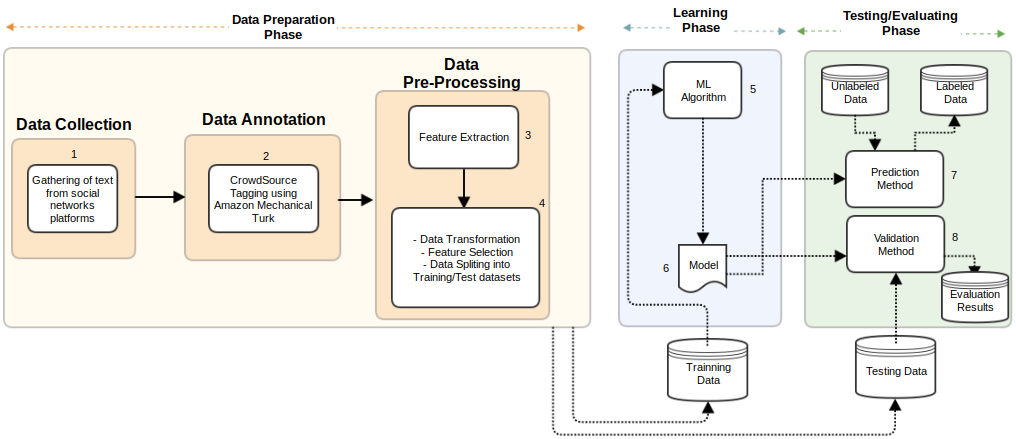
\includegraphics[scale=0.6]{./Figures/system-view/system-overview.png}
  	\rule{24cm}{0.5pt}
	\caption[System Overview]{System Overview}
	\label{fig:system-view}

\end{sidewaysfigure}

In the first stage, data from social networks is collected (1). Well-known platforms like Twitter and Facebook are be the primary sources of social content. The raw social text will then be manually annotated by people using a crowdsourcing technique. In order to achieve this, the documents are manually annotated (2). After this manual process is completed, linguistic features are extracted automatically from the texts (3). There may be data processing afterwards in order to improve the performance of the generated model (4). This stage is very important because it affects directly the performance of the chosen learning algorithm. There is an intermediate stage where a predictive model is generated through a learning algorithm (4, 5). In this case, a supervised model will be trained. NLP features will be used to extract the inputs for the ML algorithm. For instance, we may use probabilistic methods such as Bayesian Networks, search methods such as Decision Trees, optimization methods such as Support Vector Machines or even a model that combines different classifiers. \\
In the next phase, the model is tested against new data and is used to predict new relevant information. Besides, it is also important to evaluate the model using common evaluation metrics, such as precision, recall and F1, in order to extract conclusions about the performance of the model. The feedback obtained in this phase can then be used make improvements in the previous phases.\\
This work focus on the later phases of the process, that is, feature extraction and selection (3, 4), training of a predictive model (5, 6) using linguistic features extracted in the previous phase and testing and evaluation of the created model (7, 8).
The end result is a standalone classifier capable of detecting relevance from documents which might be integrated in a system.  

\section{Dataset}

%Characterization
Our experiments were supported by textual messages gathered from Twitter and Facebook, using their official APIs, in the period between the 16th to the 20th of April, 2016.
It is important to note that, during this process, text quality was preferred over text quantity.

Tweets were retrieved with the following search queries: (i)~``refugees'' and ``Syria''; (ii)~``elections'' and ``US''; (iii)~``Olympic Games''; (iv)~``terrorism''; (v)~``Daesh''; (vi)~``Referendum'' and ``UK'' and ``EU''.
The previous were selected due to their connection with topics currently discussed on the news and social networks.
Retweets were discarded.

Regarding Facebook, posts and comments were gathered from the official pages of several international news websites, namely Euronews, CNN, Washington Post, Financial Times, New York Post, The New York Times, BBC News, The Telegraph, The Guardian, The Huffington Post, Der Spiegel International, Deutsche Welle News, Pravda and Fox News.
While most of the posts would be relevant, comments would contain more diverse information, from this point of view. This would ensure that relevant and irrelevant information was kept.
Also, only documents that met the following conditions were actually used: (i)~between 8 and 100 words; (ii)~written in English; (iii)~not profanity words; (iv)~contained all the words from at least on of the search queries.

In days following their collection, the collected documents were uploaded to the CrowdFlower\footnote{\url{https://www.crowdflower.com/}} platform where an annotation task was launched.
Given a post, volunteer contributors were asked the following questions, using a 5-point Likert scale and regarding journalistic criteria:
(a)~interesting, in opposition to not interesting~(Interest) ; (b)~controversial or not~(Controversy); (c)~meaningful for a general audience in opposition to private/personal (Meaningfulness); (d)~new, in opposition to already known~(Novelty); (e)~reliable or unreliable~(Reliability); (f)~wide or narrow scope (Scope); and (g)~relevant or irrelevant~(Relevance).
To ensure some degree of quality, the texts were classified by at least three different contributors, all of them with the top Crowdflower level~(3), either from USA or UK, in order to control cultural differences. This monitoring was performed another team, belonging to the main project, responsible for the data collection.

%In this phase, we focus on the answers given for the relevance parameter.
To make our task a binary classification problem, each post had to be classified either as relevant or irrelevant.
For that purpose, the median of the answers given by the different contributors was computed and, if it was 4 or 5, the post was considered to be relevant, otherwise, irrelevant. The same method was employed for the others journalistic criteria.
Tables \ref{table-relevance-dataset},\ref{table-interesting-dataset},\ref{table-controversial-dataset},\ref{table-meaningful-dataset},\ref{table-new-dataset},\ref{table-reliable-dataset} details the number of documents grouped by social network, query and label.

%,\ref{table-dataset-fb-comments} and \ref{table-dataset-tweets} details the number of text fragments grouped by social network, search keyword and relevance label.
%Each contributor had to take at least 20 seconds to complete the task.


\begin{table*}[!htpb]
\centering
\footnotesize
\resizebox{\textwidth}{!}{%
\begin{tabular}{|l|l|l|l|l|l|l|}
\hline
\multicolumn{1}{|c|}{}
& \multicolumn{2}{c|}{\textbf{\#Facebook Posts}}
& \multicolumn{2}{c|}{\textbf{\#Facebook Comments}}
& \multicolumn{2}{c|}{\textbf{\#Tweets}} \\ \hline
\textbf{Search Word} & \textbf{Relevant} & \textbf{Irrelevant} & \textbf{Relevant} & \textbf{Irrelevant} & \textbf{Relevant} & \textbf{Irrelevant} \\
\hline
\it ``Refugees'' + ``Syria'' & 20 &  4 & 30 & 13 & 55 & 23 \\
%\hline
\it ``Elections'' + ``US' & 21 & 8 & 21 & 14 & 29 & 39 \\
%\hline
\it ``Olympic Games'' & 2 & 0 & 4 & 1 & 22 & 114 \\
%\hline
\it ``Terrorism'' & 53 & 16 & 138 & 88 & 59 & 53 \\
%\hline
\it ``Daesh'' & 2 & 0 & 14 & 12 & 26 & 30 \\
%\hline
\it ``Referendum'' + ``UK'' + ``EU'' & 4 & 0 & 7 & 1 & 14 & 4 \\
\hline
\end{tabular}%
}
\caption{Documents grouped by source, relevance label and query}
\label{table-relevance-dataset}
\end{table*}

\begin{table*}[!htpb]
\centering
\footnotesize
\resizebox{\textwidth}{!}{%
\begin{tabular}{|l|l|l|l|l|l|l|}
\hline
\multicolumn{1}{|c|}{}
& \multicolumn{2}{c|}{\textbf{\#Facebook Posts}}
& \multicolumn{2}{c|}{\textbf{\#Facebook Comments}}
& \multicolumn{2}{c|}{\textbf{\#Tweets}} \\ \hline
\textbf{Search Word} & \textbf{Interesting} & \textbf{Uninteresting} & \textbf{Interesting} & \textbf{Uninteresting} & \textbf{Interesting} & \textbf{Irrelevant} \\
\hline
\it ``Refugees'' + ``Syria'' & 21 & 3 & 30 & 13 & 55 & 23 \\
%\hline
\it ``Elections'' + ``US' & 17 & 12 & 21 & 14 & 27 & 41 \\
%\hline
\it ``Olympic Games'' & 2 & 0 & 5 & 0 & 21 & 115 \\
%\hline
\it ``Terrorism'' & 57 & 12 & 163 & 63 & 67 & 45 \\
%\hline
\it ``Daesh'' & 2 & 0 & 18 & 8 & 24 & 32 \\
%\hline
\it ``Referendum'' + ``UK'' + ``EU'' & 3 & 1 & 6 & 2 & 13 & 5 \\
\hline
\end{tabular}%
}
\caption{Documents grouped by source, interestingness label and query}
\label{table-interesting-dataset}
\end{table*}

\begin{table*}[!htpb]
\centering
\footnotesize
\resizebox{\textwidth}{!}{%
\begin{tabular}{|l|l|l|l|l|l|l|}
\hline
\multicolumn{1}{|c|}{}
& \multicolumn{2}{c|}{\textbf{\#Facebook Posts}}
& \multicolumn{2}{c|}{\textbf{\#Facebook Comments}}
& \multicolumn{2}{c|}{\textbf{\#Tweets}} \\ \hline
\textbf{Search Word} & \textbf{Controversial} & \textbf{Uncontroversial} & \textbf{Controversial} & \textbf{Uncontroversial} & \textbf{Controversial} & \textbf{Uncontroversial} \\
\hline
\it ``Refugees'' + ``Syria'' & 16 & 8 & 38 & 5 & 53 & 25 \\
%\hline
\it ``Elections'' + ``US' & 10 & 19 & 20 & 15 & 32 & 36 \\
%\hline
\it ``Olympic Games'' & 1 & 1 & 4 & 1 & 9 & 127 \\
%\hline
\it ``Terrorism'' & 44 & 25 & 186 & 40 & 74 & 38 \\
%\hline
\it ``Daesh'' & 2 & 0 & 17 & 9 & 26 & 30 \\
%\hline
\it ``Referendum'' + ``UK'' + ``EU'' & 1 & 3 & 7 & 1 & 9 & 9 \\
\hline
\end{tabular}%
}
\caption{Documents grouped by source, controversialness label and query}
\label{table-controversial-dataset}
\end{table*}

\begin{table*}[!htpb]
\centering
\footnotesize
\resizebox{\textwidth}{!}{%
\begin{tabular}{|l|l|l|l|l|l|l|}
\hline
\multicolumn{1}{|c|}{}
& \multicolumn{2}{c|}{\textbf{\#Facebook Posts}}
& \multicolumn{2}{c|}{\textbf{\#Facebook Comments}}
& \multicolumn{2}{c|}{\textbf{\#Tweets}} \\ \hline
\textbf{Search Word} & \textbf{Meaningful} & \textbf{Meaningless} & \textbf{Meaningful} & \textbf{Meaningless} & \textbf{Meaningful} & \textbf{Meaningless} \\
\hline
\it ``Refugees'' + ``Syria'' & 19 & 5 & 32 & 11 & 56 & 22 \\
%\hline
\it ``Elections'' + ``US' & 25 & 4 & 21 & 14 & 32 & 36 \\
%\hline
\it ``Olympic Games'' & 2 & 0 & 4 & 1 & 36 & 100 \\
%\hline
\it ``Terrorism'' & 59 & 10 & 152 & 74 & 62 & 50 \\
%\hline
\it ``Daesh'' & 2 & 0 & 18 & 8 & 26 & 30 \\
%\hline
\it ``Referendum'' + ``UK'' + ``EU'' & 4 & 0 & 7 & 1 & 15 & 3 \\
\hline
\end{tabular}%
}
\caption{Documents grouped by source, meaningfulness label and query}
\label{table-meaningful-dataset}
\end{table*}

\begin{table*}[!htpb]
\centering
\footnotesize
\resizebox{\textwidth}{!}{%
\begin{tabular}{|l|l|l|l|l|l|l|}
\hline
\multicolumn{1}{|c|}{}
& \multicolumn{2}{c|}{\textbf{\#Facebook Posts}}
& \multicolumn{2}{c|}{\textbf{\#Facebook Comments}}
& \multicolumn{2}{c|}{\textbf{\#Tweets}} \\ \hline
\textbf{Search Word} & \textbf{New} & \textbf{Old} & \textbf{New} & \textbf{Old} & \textbf{New} & \textbf{Old} \\
\hline
\it ``Refugees'' + ``Syria'' & 17 & 7 & 11 & 32 & 38 & 40 \\
%\hline
\it ``Elections'' + ``US' & 12 & 17 & 13 & 22 & 28 & 40 \\
%\hline
\it ``Olympic Games'' & 2 & 0 & 5 & 0 & 54 & 82 \\
%\hline
\it ``Terrorism'' & 32 & 37 & 73 & 153 & 53 & 59 \\
%\hline
\it ``Daesh'' & 1 & 1 & 7 & 19 & 29 & 27 \\
%\hline
\it ``Referendum'' + ``UK'' + ``EU'' & 2 & 2 & 2 & 6 & 12 & 6 \\
\hline
\end{tabular}%
}
\caption{Documents grouped by source, novelty label and query}
\label{table-new-dataset}
\end{table*}

\begin{table*}[!htpb]
\centering
\footnotesize
\resizebox{\textwidth}{!}{%
\begin{tabular}{|l|l|l|l|l|l|l|}
\hline
\multicolumn{1}{|c|}{}
& \multicolumn{2}{c|}{\textbf{\#Facebook Posts}}
& \multicolumn{2}{c|}{\textbf{\#Facebook Comments}}
& \multicolumn{2}{c|}{\textbf{\#Tweets}} \\ \hline
\textbf{Search Word} & \textbf{Reliable} & \textbf{Unreliable} & \textbf{Reliable} & \textbf{Unreliable} & \textbf{Reliable} & \textbf{Unreliable} \\
\hline
\it ``Refugees'' + ``Syria'' & 18 & 6 & 13 & 30 & 40 & 38 \\
%\hline
\it ``Elections'' + ``US' & 14 & 15 & 12 & 23 & 16 & 52 \\
%\hline
\it ``Olympic Games'' & 2 & 0 & 2 & 3 & 43 & 93 \\
%\hline
\it ``Terrorism'' & 41 & 28 & 61 & 165 & 34 & 78 \\
%\hline
\it ``Daesh'' & 1 & 1 & 9 & 17 & 13 & 43 \\
%\hline
\it ``Referendum'' + ``UK'' + ``EU'' & 4 & 0 & 1 & 7 & 10 & 8 \\
\hline
\end{tabular}%
}
\caption{Documents grouped by source, reliability label and query}
\label{table-reliable-dataset}
\end{table*}

\begin{table*}[!htpb]
\centering
\footnotesize
\resizebox{\textwidth}{!}{%
\begin{tabular}{|l|l|l|l|l|l|l|}
\hline
\multicolumn{1}{|c|}{}
& \multicolumn{2}{c|}{\textbf{\#Facebook Posts}}
& \multicolumn{2}{c|}{\textbf{\#Facebook Comments}}
& \multicolumn{2}{c|}{\textbf{\#Tweets}} \\ \hline
\textbf{Search Word} & \textbf{Wide} & \textbf{Narrow} & \textbf{Wide} & \textbf{Narrow} & \textbf{Wide} & \textbf{Narrow} \\
\hline
\it ``Refugees'' + ``Syria'' & 15 & 9 & 21 & 22 & 39 & 39 \\
%\hline
\it ``Elections'' + ``US' & 15 & 14 & 12 & 23 & 16 & 52 \\
%\hline
\it ``Olympic Games'' & 1 & 1 & 4 & 1 & 19 & 117 \\
%\hline
\it ``Terrorism'' & 41 & 28 & 87 & 139 & 41 & 71 \\
%\hline
\it ``Daesh'' & 2 & 0 & 10 & 16 & 15 & 41 \\
%\hline
\it ``Referendum'' + ``UK'' + ``EU'' & 3 & 1 & 0 & 8 & 9 & 9 \\
\hline
\end{tabular}%
}
\caption{Documents grouped by source, scope label and query}
\label{table-scope-dataset}
\end{table*}

In total, the data set contained 130 Facebook posts~(FB post), 343 Facebook comments~(FB comment) and 468 tweets, in a total of 941 instances. Of those, 521 text fragments were annotated as relevant, 420 as irrelevant, 552 as interesting, 389 as uninteresting, 549 as controversial, 392 as uncontroversial, 572 as meaningful, 369 as meaningless, 391 as new, 550 as old, 334 as reliable, 607 as unreliable, 350 as wide and 591 as narrow. \\
Table \ref{tab:text-examples} shows selected messages from the dataset and their source. For the same selected messages, Table~\ref{tab:label-answers} shows the answers on their labels and the resulting class.

\begin{table}[H]
\centering
\footnotesize
\begin{tabular}{|p{7cm}|l|l|}
\hline
\textbf{Content} & \textbf{Source} & \textbf{Post ID}\\
\hline
\scriptsize \it Putin: Turkey supports terrorism and stabs Russia in the back & FB post  & 1
\\
\scriptsize \it Canada to accept additional 10,000 Syrian refugees & Tweet & 2
\\
\scriptsize \it Lololol winning the internet and stomping out daesh \#merica & Tweet &3 
\\
\scriptsize \it Comparing numbers of people killed by terrorism with numbers killed by slipping in bath tub is stupid as eff. It totally ignores the mal-intent behind terrorism, its impact on way of life and ideology. & FB comment & 4
\\
\hline
\end{tabular}
\caption{Examples of messages in the dataset.}
\label{tab:text-examples}
\end{table}

\begin{table}[H]
\small
\centering
\begin{tabular}{|c|c|c|c|c|c|}
\hline
\multirow{2}{*}{\textbf{Criteria}} & \multicolumn{3}{c|}{\textbf{Answers}} & \multirow{2}{*}{\textbf{Class}} &  \multirow{2}{*}{\textbf{Post ID}} \\ \cline{2-4}
 & A1 & A2 & A3 & & \\ \hline
\multirow{4}{*}{Relevance} & 5 & 4 & 5 & Relevant & 1\\ \cline{2-6} 
 & 4 & 5 & 5 & Relevant & 2\\ \cline{2-6} 
 & 1 & 1 & 1 & Irrelevant & 3\\ \cline{2-6} 
 & 2 & 4 & 3 & Irrelevant & 4\\ \hline
 \multirow{4}{*}{Controversialness}  & 4 & 5 & 3 & Controversial & 1\\ \cline{2-6}  
 & 3 & 3 & 4 & Uncontroversial & 2 \\ \cline{2-6} 
 & 1 & 1 & 1 & Uncontroversial & 3\\ \cline{2-6}
 & 2 & 5 & 4 & Controversial & 4\\ \hline
  \multirow{4}{*}{Interestingness}  & 2 & 5 & 4 & Interesting & 1 \\ \cline{2-6} 
 & 4 & 4 & 4 & Interesting & 2\\ \cline{2-6} 
 & 1 & 1 & 1 & Uninteresting & 3\\ \cline{2-6}
 & 2 & 4 & 4 & Interesting & 4\\ \hline
  \multirow{4}{*}{Meaningfulness}  & 3 & 4 & 4 & Meaningful & 1 \\ \cline{2-6} 
 & 4 & 5 & 5 & Meaningful & 2 \\ \cline{2-6} 
 & 2 & 1 & 1 & Meaningless & 3\\ \cline{2-6}
 & 3 & 5 & 4 & Meaningful & 4\\ \hline
  \multirow{4}{*}{Novelty}  & 4 & 2 & 4 & New  & 1\\ \cline{2-6} 
 & 4 & 3 & 4 & New & 2 \\ \cline{2-6} 
 & 2 & 5 & 1 & Old & 3\\ \cline{2-6}
 & 2 & 5 & 3 & Old & 4\\ \hline
  \multirow{4}{*}{Reliability}  & 4 & 3 & 3 & Unreliable & 1 \\ \cline{2-6} 
 & 3 & 5 & 4 & Reliable & 2\\ \cline{2-6} 
 & 1 & 2 & 1 & Unreliable & 3\\ \cline{2-6}
 & 4 & 3 & 3 & Reliable & 4\\ \hline
  \multirow{4}{*}{Scope}  & 4 & 3 & 4 & Wide & 1\\ \cline{2-6} 
 & 2 & 5 & 5 & Wide & 2\\ \cline{2-6} 
 & 1 & 2 & 1 & Narrow & 3 \\ \cline{2-6}
 & 2 & 4 & 3 & Narrow & 4\\ \hline
\end{tabular}	
\caption[Answers on their labels and the resulting class]{Answers on their labels and the resulting class}
\label{tab:label-answers}
\end{table}

\section{Feature Extraction}\label{sec:features}

Our classification model was learned from a set of linguistic features extracted from each message. Initially, those were selected empirically and included: counts of PoS tags, chunk tags, NE tags and 1 to 3-grams of tokens with cutoff frequency~($f$) of 3, i.e., token n-grams that did not appear at least 3 times in the entire corpus were excluded.
We also used 1 to 5 grams of lemmatized tokens (including stopwords and punctuation signs), stems, PoS and chunk tags. Furthermore, we also included simple numerical counts such as the total number of PoS tags, chunk tags, named entities, characters, tokens, all capitalized words and their proportion in the phrase as well.
Finally, we included 3 sentiment features, namely the number of positive and negative words in the message, according to Hu and Liu's Opinion Lexicon\footnote{\url{https://www.cs.uic.edu/~liub/FBS/sentiment-analysis.html\#lexicon}}, which is a manually created lexicon that includes English words with their associated polarity, i.e., according to their perceived opinion (positive or negative). If a word was not there, it was considered to be neutral.
%Additionally, we included a typical bag-of-words in our initial feature set -- each word was treated as an unique feature with the corresponding frequency as the feature value.
Table~\ref{table-features} details the feature sets used and the distinct number of features of each kind. These features are extracted from common NLP tasks presented in section \ref{nlp_tasks} are suitable for text classification tasks\citep{scott1999feature,moschitti2004complex,Biro2008LDASpam,liu2010sentiment}.

\begin{table}[!htpb]
\centering
\footnotesize
\begin{tabular}{|l|l|}
\hline
\textbf{Feature Set} & \textbf{\#Distinct Features} 
\\
\hline
PoS-tags & 54 \\
%\hline
Chunk tags & 23 \\
%\hline
NE tags & 11 \\
%\hline
Total number of PoS/Chunk tags & 2 \\
%\hline
Total number of Named Entities & 1 \\
%\hline
Total number of positive/neutral/negative words & 3 \\
%\hline
Total number of characters/tokens & 2 \\
%\hline
Total number/proportion of all capitalized words & 2 \\
%\hline
LDA topic distribution & 20 \\
%\hline
Token 1-3grams & 2711 ($f \geq 3$ ) \\
%\hline
Lemma 1-5grams & top-750 ($f \geq 1$ ) \\
%\hline
Stem 1-5grams & top-750 ($f \geq 1$ ) \\
%\hline
PoS 1-5grams (1-5) & top-125 ($f \geq 1$ ) \\
%\hline
Chunk 1-5grams (1-5) & top-125 ($f \geq 1$ ) \\
%\hline
%Bag-of-stems & ? ($f\geq3$) \\
\hline
\textbf{Total} & 4,579 \\
%Bag-of-Words & 5,277  \\
\hline
\end{tabular}
\caption[Feature sets used]{Feature sets used}
\label{table-features}
\end{table}  

Naturally, some of the 4,579 distinct features of the initial set do not have enough discriminative power and are not distinguishing or informative enough for the classification task. Therefore, further feature selection/reduction methods should improve the quality of the final predictions.

\section{Baseline Results}
\label{sec:baseline-experiements}

This section describes baseline experiments, for detecting relevance, where we considered different sets of features and did not apply any preprocessing or feature selection method. We started with the full set of features and split the original feature set into smaller ones where only specific features were included. 

Several tools were used in our experiments. NLP features were extracted with the help of TweetNLP~\citep{Gimpel2011TweetNLP}, for PoS tagging, Twitter NLP~\citep{Ritter2011TwitterNLP}, for chunk tagging and NER, both using the pre-trained available models, and NLTK~\citep{Bird2006NLTK} for lemmatisation and stemming. For extracting n-grams, scikit-learn's\footnote{\url{http://scikit-learn.org/stable}} \citep{scikit-learn} tool  was used. Classification experiments were also performed with this machine learning toolkit. Moreover, a GUI application was developed, in Python, using PyQT5\footnote{https://pypi.python.org/pypi/PyQt5}, to aid in the execution of the different steps of the machine learning pipeline such as feature extraction, preprocessing, feature selection/reduction, classification and evaluation.

Tables \ref{tab:baseline-mdc}, \ref{tab:baseline-knn}, \ref{tab:baseline-nb}, \ref{tab:baseline-svm}, \ref{tab:baseline-dt} \ref{tab:baseline-rt} show the results of the different classification methods applied to these smaller subsets of features. Each table presents the obtained results: accuracy, precision, recall, F$_1$-score, area under the ROC curve (AUC) and average precision (AP). The minimum distance and the k-Nearest Neighbors (kNN) classifiers use the Euclidean distance as the distance metric. The number of considered neighbors was 29 since our training data contained a total of 846 instances (90\% of the dataset) and $\sqrt[]{N}$ is usually a good starting point, according to \citep{duda2012pattern}. The SVM classifier uses a linear kernel with the constant $C$ equal to 1 and the Random Forest has a total of 96 trees, which is in the middle of the range [64,128] which provides a good balance between AUC and processing time \citep{Oshiro2012}. Finally, we performed a 10-fold stratified cross validation to obtain the average results and standard deviations. 


\begin{table}[H]
\centering
\small
\resizebox{\textwidth}{!}{%
\begin{tabular}{|l|c|c|c|c|c|c|}
\hline
\multicolumn{1}{|r|}{\textbf{Classifier}} & \multicolumn{6}{c|}{\textbf{Minimum Distance Classifier}} \\ \hline
\multicolumn{1}{|r|}{\textbf{Performance Metrics}} & \multirow{2}{*}{\textbf{Accuracy}} & \multirow{2}{*}{\textbf{Precision}} & \multirow{2}{*}{\textbf{Recall}} & \multirow{2}{*}{\textbf{F$_1$}} & \multirow{2}{*}{\textbf{AP}} & \multirow{2}{*}{\textbf{AUC}} \\ \cline{1-1}
\textbf{Feature Set} &  &  &  &  &  &  \\ \hline
Full feature set &  0.57 $\pm$ 0.05 & \textbf{0.72 $\pm$ 0.14} & 0.41 $\pm$ 0.14 & 0.50 $\pm$ 0.11 & 0.73 $\pm$ 0.07 & 0.59 $\pm$ 0.05 \\ \hline
Part-of-speech & 0.57 $\pm$ 0.06 & 0.71 $\pm$ 0.15 & 0.42 $\pm$ 0.14 & 0.50 $\pm$ 0.11 & 0.72 $\pm$ 0.07 & 0.58 $\pm$ 0.06 \\ \hline
Chunks & 0.57 $\pm$ 0.05 & 0.71 $\pm$ 0.14 & 0.42 $\pm$ 0.13 & 0.51 $\pm$ 0.10 & 0.72 $\pm$ 0.07 & 0.59 $\pm$ 0.05 \\ \hline
Named entities & 0.57 $\pm$ 0.05 & 0.71 $\pm$ 0.14 & 0.42 $\pm$ 0.13 & 0.51 $\pm$ 0.10 & 0.72 $\pm$ 0.07 & 0.58 $\pm$ 0.05 \\ \hline
Chars+Tokens+Allcaps+Allcaps-ratio & 0.57 $\pm$ 0.06 & 0.71 $\pm$ 0.14 & 0.41 $\pm$ 0.14 & 0.50 $\pm$ 0.11 & 0.73 $\pm$ 0.07 & 0.59 $\pm$ 0.05 \\ \hline
Positive+Neutral+Negative & 0.56 $\pm$ 0.05 & 0.70 $\pm$ 0.15 & 0.41 $\pm$ 0.13 & 0.50 $\pm$ 0.11 & 0.72 $\pm$ 0.07 & 0.58 $\pm$ 0.05 \\ \hline
LDA topic distribution & \textbf{0.63 $\pm$ 0.15} & 0.65 $\pm$ 0.17 & \textbf{0.89 $\pm$ 0.17} & \textbf{0.73 $\pm$ 0.12} &\textbf{ 0.80 $\pm$ 0.09} & \textbf{0.60 $\pm$ 0.17} \\ \hline
Token n-grams & 0.57 $\pm$ 0.06 & 0.70 $\pm$ 0.16 & 0.46 $\pm$ 0.15 & 0.53 $\pm$ 0.11 & 0.73 $\pm$ 0.08 & 0.58 $\pm$ 0.06 \\ \hline
Lemma n-grams & 0.58 $\pm$ 0.05 & 0.71 $\pm$ 0.14 & 0.48 $\pm$ 0.15 & 0.55 $\pm$ 0.10 & 0.74 $\pm$ 0.07 & \textbf{0.60 $\pm$ 0.05} \\ \hline
Stem n-grams & 0.59 $\pm$ 0.05 & \textbf{0.72 $\pm$ 0.13} & 0.48 $\pm$ 0.15 & 0.55 $\pm$ 0.10 & 0.74 $\pm$ 0.06 & \textbf{0.60 $\pm$ 0.05} \\ \hline
PoS n-grams & 0.58 $\pm$ 0.05 & 0.71 $\pm$ 0.11 & 0.46 $\pm$ 0.16 & 0.53 $\pm$ 0.12 & 0.73 $\pm$ 0.05 & 0.59 $\pm$ 0.05 \\ \hline
Chunk n-grams & 0.57 $\pm$ 0.06 & 0.70 $\pm$ 0.15 & 0.43 $\pm$ 0.14 & 0.51 $\pm$ 0.11 & 0.72 $\pm$ 0.07 & 0.59 $\pm$ 0.05 \\ \hline
\end{tabular}%
}
\caption[Baseline Results for the Minimum Distance Classifier]{Baseline Results for the Minimum Distance Classifier}
\label{tab:baseline-mdc}
\end{table}

\begin{table}[H]
\centering
\small
\resizebox{\textwidth}{!}{%
\begin{tabular}{|l|c|c|c|c|c|c|}
\hline
\multicolumn{1}{|r|}{\textbf{Classifier}} & \multicolumn{6}{c|}{\textbf{k-Nearest Neighbors (kNN)}} \\ \hline
\multicolumn{1}{|r|}{\textbf{Performance Metrics}} & \multirow{2}{*}{\textbf{Accuracy}} & \multirow{2}{*}{\textbf{Precision}} & \multirow{2}{*}{\textbf{Recall}} & \multirow{2}{*}{\textbf{F$_1$}} & \multirow{2}{*}{\textbf{AP}} & \multirow{2}{*}{\textbf{AUC}} \\ \cline{1-1}
\textbf{Feature Set} &  &  &  &  &  &  \\ \hline
Full feature set & 0.57 $\pm$ 0.05 & 0.60 $\pm$ 0.05 & 0.73$\pm$ 0.12 & 0.65 $\pm$ 0.05 & 0.74 $\pm$ 0.03 & 0.55 $\pm$ 0.06 \\ \hline
Part-of-speech & 0.60 $\pm$ 0.06 & 0.61 $\pm$ 0.05 & 0.83 $\pm$ 0.09 & 0.70 $\pm$ 0.05 & 0.77 $\pm$ 0.03 & 0.58 $\pm$ 0.07 \\ \hline
Chunks & 0.58 $\pm$ 0.04 & 0.58 $\pm$ 0.04 & 0.76 $\pm$ 0.09 & 0.67 $\pm$ 0.04 & 0.75 $\pm$ 0.03 & 0.56 $\pm$ 0.05 \\ \hline
Named entities & 0.58 $\pm$ 0.07 & 0.62 $\pm$ 0.08 & 0.71 $\pm$ 0.11 & 0.65 $\pm$ 0.06 & 0.74 $\pm$ 0.05 & 0.57 $\pm$ 0.08  \\ \hline
Chars+Tokens+Allcaps+Allcaps-ratio & 0.57 $\pm$ 0.06 & 0.60 $\pm$ 0.05 & 0.70 $\pm$ 0.09 & 0.64 $\pm$ 0.05 & 0.73 $\pm$ 0.03 & 0.55 $\pm$ 0.06 \\ \hline
Positive+Neutral+Negative & 0.54 $\pm$ 0.06 & 0.58 $\pm$ 0.04 & 0.62 $\pm$ 0.15 & 0.59 $\pm$ 0.09 & 0.71 $\pm$ 0.05 & 0.53 $\pm$ 0.05 \\ \hline
LDA topic distribution & \textbf{0.62 $\pm$ 0.12} & 0.64 $\pm$ 0.13 & \textbf{0.85 $\pm$ 0.13} & \textbf{0.72 $\pm$ 0.09} & \textbf{0.79 $\pm$ 0.07} & \textbf{0.60 $\pm$ 0.14} \\ \hline
Token n-grams & 0.51 $\pm$ 0.05 & \textbf{0.72 $\pm$ 0.15} & 0.20 $\pm$ 0.09 & 0.30 $\pm$ 0.11 & 0.68 $\pm$ 0.08 & 0.55 $\pm$ 0.04 \\ \hline
Lemma n-grams & 0.59 $\pm$ 0.09 & 0.70 $\pm$ 0.14 & 0.47 $\pm$ 0.12 & 0.55 $\pm$ 0.11 & 0.73 $\pm$ 0.09 & \textbf{0.60 $\pm$ 0.09} \\ \hline
Stem n-grams & 0.57 $\pm$ 0.08 & 0.69 $\pm$ 0.15 & 0.43 $\pm$ 0.13 & 0.52 $\pm$ 0.12 & 0.72 $\pm$ 0.09 & 0.59 $\pm$ 0.08 \\ \hline
PoS n-grams & 0.58 $\pm$ 0.05 & 0.61 $\pm$ 0.05 & 0.61 $\pm$ 0.05 & 0.66 $\pm$ 0.06 & 0.74 $\pm$ 0.04 & 0.56 $\pm$ 0.06 \\ \hline
Chunk n-grams & 0.57 $\pm$ 0.05 & 0.60 $\pm$ 0.04 & 0.67 $\pm$ 0.10 & 0.63 $\pm$ 0.05 & 0.73 $\pm$ 0.03 & 0.55 $\pm$ 0.05 \\ \hline
\end{tabular}%
}
\caption[Baseline Results for the k-Nearest Neighbor Classifier]{Baseline Results for the k-Nearest Neighbor Classifier}
\label{tab:baseline-knn}
\end{table}

\begin{table}[H]
\centering
\small
\resizebox{\textwidth}{!}{%
\begin{tabular}{|l|c|c|c|c|c|c|}
\hline
\multicolumn{1}{|r|}{\textbf{Classifier}} & \multicolumn{6}{c|}{\textbf{Naive Bayes}} \\ \hline
\multicolumn{1}{|r|}{\textbf{Performance Metrics}} & \multirow{2}{*}{\textbf{Accuracy}} & \multirow{2}{*}{\textbf{Precision}} & \multirow{2}{*}{\textbf{Recall}} & \multirow{2}{*}{\textbf{F$_1$}} & \multirow{2}{*}{\textbf{AP}} & \multirow{2}{*}{\textbf{AUC}} \\ \cline{1-1}
\textbf{Feature Set} &  &  &  &  &  &  \\ \hline
Full feature set & 0.60 $\pm$ 0.11 & 0.63 $\pm$ 0.11 & 0.73 $\pm$ 0.16 & 0.66 $\pm$ 0.12 & 0.75 $\pm$ 0.08 & 0.59 $\pm$ 0.12 \\ \hline
Part-of-speech & 0.58 $\pm$ 0.07 & 0.70 $\pm$ 0.13 & 0.33 $\pm$ 0.11 & 0.44 $\pm$ 0.10 & 0.70 $\pm$ 0.07 & 0.57 $\pm$ 0.05 \\ \hline
Chunks & 0.46 $\pm$ 0.03 & 0.50 $\pm$ 0.30 & 0.07 $\pm$ 0.06 & 0.12 $\pm$ 0.09 & 0.64 $\pm$ 0.11 & 0.51 $\pm$ 0.03 \\ \hline
Named entities & 0.58 $\pm$ 0.09 & 0.58 $\pm$ 0.09 & 0.77 $\pm$ 0.11 & 0.67 $\pm$ 0.06 & 0.75 $\pm$ 0.04 & 0.55 $\pm$ 0.10 \\ \hline
Chars+Tokens+Allcaps+Allcaps-ratio & 0.57 $\pm$ 0.04 & 0.57 $\pm$ 0.02 & \textbf{0.93 $\pm$ 0.07} & 0.70 $\pm$ 0.03 & 0.77 $\pm$ 0.02 & 0.53 $\pm$ 0.04 \\ \hline
Positive+Neutral+Negative & 0.55 $\pm$ 0.06 & 0.69 $\pm$ 0.12 & 0.34 $\pm$ 0.12 & 0.44 $\pm$ 0.12 & 0.70 $\pm$ 0.07 & 0.57 $\pm$ 0.05 \\ \hline
LDA topic distribution & \textbf{0.64 $\pm$ 0.13} & 0.67 $\pm$ 0.16 & 0.82 $\pm$ 0.13 & \textbf{0.72 $\pm$ 0.10} & \textbf{0.79 $\pm$ 0.08} & \textbf{0.62 $\pm$ 0.15} \\ \hline
Token n-grams & 0.61 $\pm$ 0.11 & 0.63 $\pm$ 0.11 & 0.71 $\pm$ 0.16 & 0.66 $\pm$ 0.11 & 0.75 $\pm$ 0.08 & 0.59 $\pm$ 0.11 \\ \hline
Lemma n-grams & 0.59 $\pm$ 0.10 & 0.68 $\pm$ 0.15 & 0.54 $\pm$ 0.12 & 0.59 $\pm$ 0.11 & 0.74 $\pm$ 0.08 & 0.60 $\pm$ 0.10 \\ \hline
Stem n-grams & 0.60 $\pm$ 0.09 & 0.68 $\pm$ 0.14 & 0.56 $\pm$ 0.12 & 0.60 $\pm$ 0.11 & 0.74 $\pm$ 0.08 & 0.60 $\pm$ 0.10 \\ \hline
PoS n-grams & 0.58 $\pm$ 0.06 & \textbf{0.70 $\pm$ 0.15} & 0.48 $\pm$ 0.17 & 0.54 $\pm$ 0.12 & 0.74 $\pm$ 0.07 & 0.59 $\pm$ 0.06 \\ \hline
Chunk n-grams & 0.56 $\pm$ 0.05 & 0.69 $\pm$ 0.12 & 0.42 $\pm$ 0.13 & 0.50 $\pm$ 0.10 & 0.71 $\pm$ 0.06 & 0.58 $\pm$ 0.05 \\ \hline
\end{tabular}%
}
\caption[Baseline Results for the Naive Bayes Classifier]{Baseline Results for the Naive Bayes Classifier}
\label{tab:baseline-nb}
\end{table}

\begin{table}[H]
\centering
\small
\resizebox{\textwidth}{!}{%
\begin{tabular}{|l|c|c|c|c|c|c|}
\hline
\multicolumn{1}{|r|}{\textbf{Classifier}} & \multicolumn{6}{c|}{\textbf{Support Vector Machine (SVM)}} \\ \hline
\multicolumn{1}{|r|}{\textbf{Performance Metrics}} & \multirow{2}{*}{\textbf{Accuracy}} & \multirow{2}{*}{\textbf{Precision}} & \multirow{2}{*}{\textbf{Recall}} & \multirow{2}{*}{\textbf{F$_1$}} & \multirow{2}{*}{\textbf{AP}} & \multirow{2}{*}{\textbf{AUC}} \\ \cline{1-1}
\textbf{Feature Set} &  &  &  &  &  &  \\ \hline
Full feature set & 0.60 $\pm$ 0.10 & \textbf{0.67 $\pm$ 0.14} & 0.63 $\pm$ 0.08 & 0.64 $\pm$ 0.08 & 0.75 $\pm$ 0.07 & 0.60 $\pm$ 0.11 \\ \hline
Part-of-speech & 0.63 $\pm$ 0.08 & 0.66 $\pm$ 0.09 & 0.71 $\pm$ 0.21 & 0.66 $\pm$ 0.12 & 0.76 $\pm$ 0.06 & \textbf{0.62 $\pm$ 0.08} \\ \hline
Chunks & 0.58 $\pm$ 0.07 & 0.59 $\pm$ 0.05 & 0.75 $\pm$ 0.24 & 0.64 $\pm$ 0.15 & 0.64 $\pm$ 0.15 & 0.56 $\pm$ 0.06 \\ \hline
Named entities & 0.55 $\pm$ 0.09 & 0.51 $\pm$ 0.29 & 0.64 $\pm$ 0.42 & 0.51 $\pm$ 0.32 & 0.78 $\pm$ 0.03 & 0.54 $\pm$ 0.07 \\ \hline
Chars+Tokens+Allcaps+Allcaps-ratio & 0.54 $\pm$ 0.06 & 0.45 $\pm$ 0.23 & 0.74 $\pm$ 0.38 & 0.56 $\pm$ 0.28 & 0.77 $\pm$ 0.02 & 0.51 $\pm$ 0.04 \\ \hline
Positive+Neutral+Negative & 0.52 $\pm$ 0.05 & 0.59 $\pm$ 0.26 & 0.60 $\pm$ 0.40 & 0.48 $\pm$ 0.29 & 0.71 $\pm$ 0.15 & 0.51 $\pm$ 0.02 \\ \hline
LDA topic distribution & \textbf{0.64 $\pm$ 0.14} & 0.65 $\pm$ 0.16 & \textbf{0.85 $\pm$ 0.19} & \textbf{0.72 $\pm$ 0.13} & \textbf{0.79 $\pm$ 0.09} & 0.61 $\pm$ 0.16 \\ \hline
Token n-grams & 0.60 $\pm$ 0.09 & 0.65 $\pm$ 0.11 & 0.62 $\pm$ 0.11 & 0.63 $\pm$ 0.09 & 0.74 $\pm$ 0.06 & 0.59 $\pm$ 0.09 \\ \hline
Lemma n-grams & 0.59 $\pm$ 0.07 & 0.65 $\pm$ 0.11 & 0.61 $\pm$ 0.08 & 0.62 $\pm$ 0.06 & 0.74 $\pm$ 0.05 & 0.58 $\pm$ 0.08 \\ \hline
Stem n-grams & 0.61 $\pm$ 0.09 & 0.69 $\pm$ 0.14 & 0.62 $\pm$ 0.11 & 0.64 $\pm$ 0.08 & 0.76 $\pm$ 0.07 & 0.61 $\pm$ 0.09 \\ \hline
PoS n-grams & 0.58 $\pm$ 0.09 & 0.63 $\pm$ 0.12 & 0.63 $\pm$ 0.15 & 0.62 $\pm$ 0.11 & 0.73 $\pm$ 0.08 & 0.58 $\pm$ 0.10 \\ \hline
Chunk n-grams & 0.56 $\pm$ 0.06 & 0.59 $\pm$ 0.05 & 0.69 $\pm$ 0.17 & 0.62 $\pm$ 0.09 & 0.72 $\pm$ 0.05 & 0.54 $\pm$ 0.05 \\ \hline
\end{tabular}%
}
\caption[Baseline Results for the Support Vector Machine Classifier ]{Baseline Results for the Support Vector Machine Classifier}
\label{tab:baseline-svm}
\end{table}

\begin{table}[H]
\centering
\small
\resizebox{\textwidth}{!}{%
\begin{tabular}{|l|c|c|c|c|c|c|}
\hline
\multicolumn{1}{|r|}{\textbf{Classifier}} & \multicolumn{6}{c|}{\textbf{Decision Tree}} \\ \hline
\multicolumn{1}{|r|}{\textbf{Performance Metrics}} & \multirow{2}{*}{\textbf{Accuracy}} & \multirow{2}{*}{\textbf{Precision}} & \multirow{2}{*}{\textbf{Recall}} & \multirow{2}{*}{\textbf{F$_1$}} & \multirow{2}{*}{\textbf{AP}} & \multirow{2}{*}{\textbf{AUC}} \\ \cline{1-1}
\textbf{Feature Set} &  &  &  &  &  &  \\ \hline
Full feature set & 0.58 $\pm$ 0.05 & 0.63 $\pm$ 0.08 & \textbf{0.63 $\pm$ 0.09} & 0.62 $\pm$ 0.05 & 0.73 $\pm$ 0.04 & 0.57 $\pm$ 0.06  \\ \hline
Part-of-speech & 0.57 $\pm$ 0.08 & 0.62 $\pm$ 0.09 & 0.60 $\pm$ 0.06 & 0.61 $\pm$ 0.05 & 0.72 $\pm$ 0.05 & 0.56 $\pm$ 0.08 \\ \hline
Chunks & 0.55 $\pm$ 0.04 & 0.59 $\pm$ 0.04 & 0.59 $\pm$ 0.06 & 0.59 $\pm$ 0.04 & 0.71 $\pm$ 0.03 & 0.54 $\pm$ 0.04 \\ \hline
Named entities & 0.53 $\pm$ 0.04 & 0.58 $\pm$ 0.04 &  0.55 $\pm$ 0.05 & 0.57 $\pm$ 0.04 & 0.69 $\pm$ 0.02 & 0.53 $\pm$ 0.04 \\ \hline
Chars+Tokens+Allcaps+Allcaps-ratio & 0.55 $\pm$ 0.04 & 0.59 $\pm$ 0.04 & 0.61 $\pm$ 0.07 & 0.60 $\pm$ 0.05 & 0.71 $\pm$ 0.03 & 0.54 $\pm$ 0.04 \\ \hline
Positive+Neutral+Negative & 0.53 $\pm$ 0.04 & 0.58 $\pm$ 0.04 & 0.51 $\pm$ 0.10 & 0.54 $\pm$ 0.07 & 0.68 $\pm$ 0.04 & 0.53 $\pm$ 0.04 \\ \hline
LDA topic distribution & 0.55 $\pm$ 0.07 & 0.60 $\pm$ 0.09 & 0.58 $\pm$ 0.08 & 0.59 $\pm$ 0.06 & 0.71 $\pm$ 0.05 & 0.54 $\pm$ 0.08 \\ \hline
Token n-grams & 0.55 $\pm$ 0.12 & 0.61 $\pm$ 0.14 & 0.61 $\pm$ 0.13 & 0.60 $\pm$ 0.11 & 0.72 $\pm$ 0.08 & 0.54 $\pm$ 0.13 \\ \hline
Lemma n-grams & 0.57 $\pm$ 0.10 & 0.63 $\pm$ 0.13 & 0.61 $\pm$ 0.11 & 0.61 $\pm$ 0.09 & 0.73 $\pm$ 0.08 & 0.57 $\pm$ 0.10 \\ \hline
Stem n-grams & 0.56 $\pm$ 0.08 & 0.62 $\pm$ 0.12 & 0.58 $\pm$ 0.10 & 0.59 $\pm$ 0.07 & 0.72 $\pm$ 0.06 &  0.55 $\pm$ 0.08\\ \hline
PoS n-grams & \textbf{0.60 $\pm$ 0.06} & \textbf{0.64 $\pm$ 0.06} & 0.62 $\pm$ 0.08 & \textbf{0.63 $\pm$ 0.06} & \textbf{0.74 $\pm$ 0.04} & \textbf{0.59 $\pm$ 0.06} \\ \hline
Chunk n-grams & 0.56 $\pm$ 0.06 & 0.61 $\pm$ 0.06 & 0.59 $\pm$ 0.08 & 0.60 $\pm$ 0.06 & 0.71 $\pm$ 0.04 & 0.56 $\pm$ 0.06
 \\ \hline
\end{tabular}%
}
\caption[Baseline Results for the Decision Tree Classifier]{Baseline Results for the Decision Tree Distance Classifier}
\label{tab:baseline-dt}
\end{table}

\begin{table}[H]
\centering
\small
\resizebox{\textwidth}{!}{%
\begin{tabular}{|l|c|c|c|c|c|c|}
\hline
\multicolumn{1}{|r|}{\textbf{Classifier}} & \multicolumn{6}{c|}{\textbf{Random Forest Classifier }} \\ \hline
\multicolumn{1}{|r|}{\textbf{Performance Metrics}} & \multirow{2}{*}{\textbf{Accuracy}} & \multirow{2}{*}{\textbf{Precision}} & \multirow{2}{*}{\textbf{Recall}} & \multirow{2}{*}{\textbf{F$_1$}} & \multirow{2}{*}{\textbf{AP}} & \multirow{2}{*}{\textbf{AUC}} \\ \cline{1-1}
\textbf{Feature Set} &  &  &  &  &  &  \\ \hline
Full feature set & \textbf{0.64 $\pm$ 0.06} & 0.66 $\pm$ 0.09 & \textbf{0.78 $\pm$ 0.10} & \textbf{0.71 $\pm$ 0.04} & 0.78 $\pm$ 0.04 & \textbf{0.62 $\pm$ 0.09} \\ \hline
Part-of-speech & 0.63 $\pm$ 0.07 & 0.66 $\pm$ 0.09 & \textbf{0.78 $\pm$ 0.11} & 0.70 $\pm$ 0.05 & 0.78 $\pm$ 0.04 & \textbf{0.62 $\pm$ 0.08} \\ \hline
Chunks & 0.60 $\pm$ 0.04 & 0.62 $\pm$ 0.04 & 0.70 $\pm$ 0.07 & 0.66 $\pm$ 0.04 & 0.74 $\pm$ 0.02 & 0.58 $\pm$ 0.04 \\ \hline
Named entities & 0.58 $\pm$ 0.06 & 0.62 $\pm$ 0.06 & 0.66 $\pm$ 0.07 & 0.64 $\pm$ 0.05 & 0.73 $\pm$ 0.04 & 0.56 $\pm$ 0.06 \\ \hline
Chars+Tokens+Allcaps+Allcaps-ratio & 0.55 $\pm$ 0.03 & 0.59 $\pm$ 0.03 & 0.61 $\pm$ 0.09 & 0.60 $\pm$ 0.05 & 0.71 $\pm$ 0.03 & 0.54 $\pm$ 0.03 \\ \hline
Positive+Neutral+Negative & 0.52 $\pm$ 0.04 & 0.57 $\pm$ 0.03 & 0.57 $\pm$ 0.09 & 0.57 $\pm$ 0.05 & 0.69 $\pm$ 0.03 & 0.51 $\pm$ 0.04 \\ \hline
LDA topic distribution & 0.60 $\pm$ 0.11 & 0.65 $\pm$ 0.16 & 0.75 $\pm$ 0.15 & 0.67 $\pm$ 0.10 & 0.77 $\pm$ 0.08 & 0.58 $\pm$ 0.13	 \\ \hline
Token n-grams & 0.62 $\pm$ 0.10 & 0.66 $\pm$ 0.15 & 0.77 $\pm$ 0.16 & 0.69 $\pm$ 0.09 & 0.78 $\pm$ 0.07 & 0.60 $\pm$ 0.12 \\ \hline
Lemma n-grams & 0.63 $\pm$ 0.11 & 0.66 $\pm$ 0.16 & \textbf{0.78 $\pm$ 0.13} & 0.70 $\pm$ 0.09 & 0.78 $\pm$ 0.08 & 0.61 $\pm$ 0.13 \\ \hline
Stem n-grams & 0.64 $\pm$ 0.11 & \textbf{0.67 $\pm$ 0.15} & 0.78 $\pm$ 0.16 & 0.70 $\pm$ 0.10 & \textbf{0.79 $\pm$ 0.08} & \textbf{0.62 $\pm$ 0.12} \\ \hline
PoS n-grams & 0.62 +- 0.06 & 0.65 +- 0.10 & 0.77 +- 0.11 & 0.69 +- 0.04 & 0.77 +- 0.04 & 0.61 +- 0.08 \\ \hline
Chunk n-grams & 0.59 $\pm$ 0.04 & 0.59 $\pm$ 0.04 & 0.72 $\pm$ 0.10 & 0.66 $\pm$ 0.05 & 0.74 $\pm$ 0.03 & 0.57 $\pm$ 0.05 \\ \hline
\end{tabular}%
}
\caption[Baseline Results for the Random Forest Classifier]{Baseline Results for the Random Forest Classifier}
\label{tab:baseline-rt}
\end{table}

% Considering the full feature set, the Random Forest obtained the best accuracy(0.64). Surprisingly, the Minimum Distance Classifier obtained the best precision(0.72). The Random Forest got the best recall(0.78) while the kNN got the best F$_1$(0.66). The Random Forest obtained the best areas under the roc and precision-recall curves, obtaining (0.75) and (0.62), respectively, closely followed by the SVM classifier.

% Regarding the PoS tags, both SVM and Random Forest obtained an accuracy of 0.63, while the Minimum Distance Classifier got a precision of 0.71  and the kNN got the best recall(0.83). In respect to the F$1$ measure, both kNN and Random Forest obtained 0.70. The SVM classifier achieved the same result as the Random Forest regarding average precision(0.62) while the Random Forest obtained the best AUC(0.78).

The Naive Bayes and the SVM classier achieve the best accuracy(0.64) on the set consisting of LDA topics. The Minimum Distance Classifier obtained the best precisions(0.72) using the full dataset and n-grams of stems while the kNN classifier achieved also the same precision(0.72) using ngams of tokens. The LDA topic distribution proved to be a good feature set, achieving the best recall(0.89), F$_1$ score(0.73) and average precision(0.80) using a Minimum Distance Classifier. In fact, it is possible that some topic distributions were more likely to be associated with relevant data (or irrelevant) and be highly influenced by some typical words. However, the Naive Bayes, the SVM and the Random Forest obtained the best area under the ROC curve(0.62). To achieve this AUC, the Naive Bayes used the LDA topics, the SVM used the PoS tags and the Random Forest achieved the same result by using the full feature set, PoS tags and stem ngrams. 
Surprisingly, for such a simple model such as the Minimum Distance Classifier, it got fairly good results, suggesting that the distance between mean feature vectors is large enough to discriminate both classes. The Random Forest, kNN and the Naive Bayes always competed against the best results, while the Decision Tree did not performed so well, achieving results just a little above a random classifier. Another important note is that small subsets such as the countings of characters/tokens/allcaps/allcaps-ratio (4 features) were sometimes enough to make decent predictions. For example, using this small set, the Naive Bayes achieved a F$_1$ score of 0.70. On the other, the polarity set did not performed very well.  Although some feature sets work better in some cases and worse in others, this suggest that a combination of the most informative features from each set may improve the classification results. 

\begin{figure}[H]
	\centering
	\resizebox{\textwidth}{!}{
  	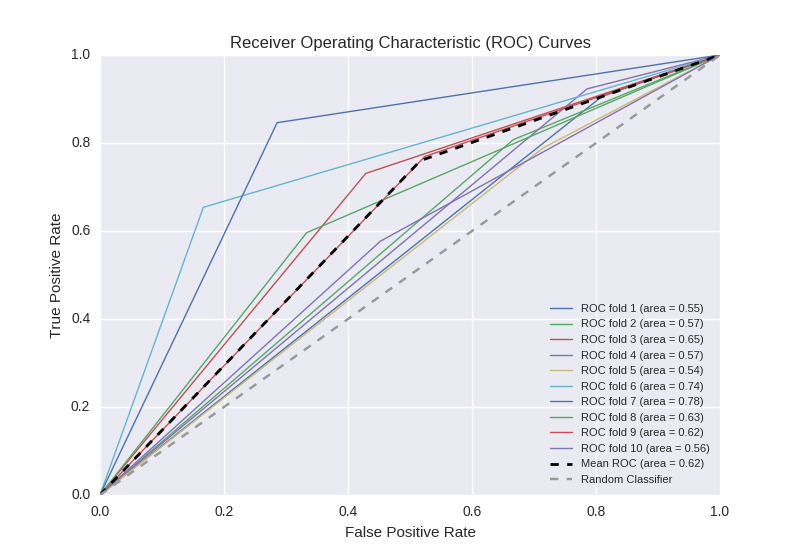
\includegraphics{./Figures/experiments/baseline/roc}
     }
	\caption[ROC Curves of a SVM  Classifier using PoS tags as features]{ROC Curves of a SVM  Classifier using PoS tags as features}
	\label{fig:baseline-roc-svm-pos}
\end{figure}

\begin{figure}[H]
	\centering
	\resizebox{\textwidth}{!}{
  	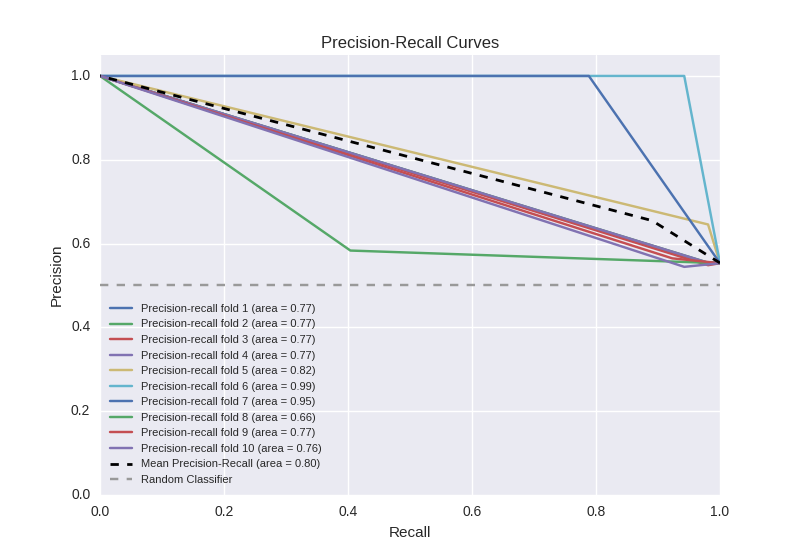
\includegraphics{./Figures/experiments/baseline/pr_curve}
     }
	\caption[Precision-Recall Curves of a Minimum Distance Classifier using LDA topic distributions as features]{Precision-Recall Curves of a Minimum Distance Classifier using LDA topic distributions as features}
	\label{fig:baseline-pr-mdc-lda}
\end{figure}

Figure \ref{fig:baseline-roc-svm-pos} shows the best average ROC curve obtained by a SVM classifier. For low false positive rates ($<$ 0.20), the SVM classifier achieves true positive rates a little better random. However, if we are allowed to increase the false positive rate, the the number of correctly identified instances increases, achieving true positive rates $>$ 0.80 in some cases. Figure \ref{fig:baseline-pr-mdc-lda} shows the best average Precision-Recall curves obtained by a Minimum Distance Classifier. It consistently shows fairy good trade-offs between the obtained precision and recall values, achieving areas greater than $0.90$ in some cases. 



%%%%%%%%%%%%%%%%%%%%%%%%%%%%%%%%%%%%%%%%%%%%%%%%%%%%%%%%%%%%%%%%%%%%%%%%%%%%%%%%%%%%%%%%%%%%%%%%%%%%%%%%%%%%%%%%%%
\section{Feature Engineering Results}
\label{sec:feature-engineering}

Successful removal of noisy and redundant data typically improves the overall classification accuracy of the resulting model, reducing also overfitting. For this purpose, we used different preprocessing methods such as: Standardization, Normalization and Scaling and feature selection methods such as: information gain, gain ratio, chi-square ($\chi^2$), Fisher Score, Pearson correlations and feature reduction techniques such as principal component analysis. The PCA method was applied to 4 dimensions and the Pearson correlations were used to exclude features that did not have a correlation of at least $0.2$ with the target class. The classifiers were used with the same parameterization of the baseline experiments. The 10-fold cross validation was performed as well, where the feature selection/reduction methods were performed within each fold, using only the training set, in order to avoid the feature selection methods using information from the test set, such as labels, and thus avoiding bias. \\
In order to choose the number $f$ of features we followed a very simple heuristic. We applied the $\chi^2$ statistic test to find the number of statistically significant features, i.e., features that had a statistic score of $\chi^2 > 10.83$, meaning that they are very likely to be dependent from the target class, with only a $0.001$ chance of being wrong. The obtained size was $f = 210$ and it was the number of selected features. Tables \ref{tab:fe-mdc},\ref{tab:fe-knn},\ref{tab:fe-nb},\ref{tab:fe-svm},\ref{tab:fe-dt} and \ref{tab:fe-rt} show the obtained results for each classifier in predicting relevance.

\begin{table}[H]
\centering
\small
\resizebox{\textwidth}{!}{%
\begin{tabular}{|l|c|c|c|c|c|c|}
\hline
\multicolumn{1}{|r|}{\textbf{Classifier}} & \multicolumn{6}{c|}{\textbf{Minimum Distance Classifier }} \\ \hline
\multicolumn{1}{|r|}{\textbf{Performance Metrics}} & \multirow{2}{*}{\textbf{Accuracy}} & \multirow{2}{*}{\textbf{Precision}} & \multirow{2}{*}{\textbf{Recall}} & \multirow{2}{*}{\textbf{F$_1$}} & \multirow{2}{*}{\textbf{AP}} & \multirow{2}{*}{\textbf{AUC}} \\ \cline{1-1}
\textbf{Pipeline applied} &  &  &  &  &  &  \\ \hline
Standardization + full feature set & 0.57 $\pm$ 0.05 & \textbf{0.72 $\pm$ 0.14} & 0.41 $\pm$ 0.14 & 0.50 $\pm$ 0.11 & 0.73 $\pm$ 0.07 & 0.59 $\pm$ 0.05 \\ \hline
Normalization + full feature set & 0.57 $\pm$ 0.05 & \textbf{0.72 $\pm$ 0.14} & 0.41 $\pm$ 0.14 & 0.50 $\pm$ 0.11 & 0.73 $\pm$ 0.07 & 0.59 $\pm$ 0.05 \\ \hline
Scaling[0,1] + full feature set & 0.57 $\pm$ 0.05 & \textbf{0.72 $\pm$ 0.14} & 0.41 $\pm$ 0.14 & 0.50 $\pm$ 0.11 & 0.73 $\pm$ 0.07 & 0.59 $\pm$ 0.05 \\ \hline
Standardization + information gain& 0.57 $\pm$ 0.05 & \textbf{0.72 $\pm$ 0.14} & 0.41 $\pm$ 0.14 & 0.50 $\pm$ 0.11 & 0.73 $\pm$ 0.07 & 0.59 $\pm$ 0.05 \\ \hline
Standardization + gain ratio& 0.57 $\pm$ 0.05 & 0.58 $\pm$ 0.06 & \textbf{0.86 $\pm$ 0.17} & \textbf{0.68 $\pm$ 0.05} & \textbf{0.76 $\pm$ 0.04} & 0.53 $\pm$ 0.07 \\ \hline
Standardization + chi square ($\chi^2$)& 0.57 $\pm$ 0.05 & \textbf{0.72 $\pm$ 0.14} & 0.41 $\pm$ 0.14 & 0.50 $\pm$ 0.11 & 0.73 $\pm$ 0.07 & 0.59 $\pm$ 0.05 \\ \hline
Standardization + fisher score& 0.51 $\pm$ 0.07 & 0.62 $\pm$ 0.17 & 0.32 $\pm$ 0.13 & 0.41 $\pm$ 0.11 & 0.66 $\pm$ 0.09 & 0.53 $\pm$ 0.08 \\ \hline
Standardization + pearson & \textbf{0.65 $\pm$ 0.16} & 0.70 $\pm$ 0.15 & 0.63 $\pm$ 0.20 & 0.65 $\pm$ 0.18 & 0.77 $\pm$ 0.11 & \textbf{0.62 $\pm$ 0.16} \\ \hline
Standardization + pearson + pca4d& \textbf{0.65 $\pm$ 0.16} & 0.70 $\pm$ 0.15 & 0.63 $\pm$ 0.20 & 0.65 $\pm$ 0.18 & 0.77 $\pm$ 0.11 & \textbf{0.62 $\pm$ 0.16} \\ \hline
Standardization + gain ratio + pca4d & 0.57 $\pm$ 0.07 & 0.55 $\pm$ 0.08 &\textbf{0.86 $\pm$ 0.29} & 0.65 $\pm$ 0.19 & 0.75 $\pm$ 0.10 & 0.53 $\pm$ 0.06 \\ \hline
\end{tabular}%
}
\caption[Results of applying different Preprocessing and Feature Selection methods with a Minimum Distance Classifier]{Results of applying different Preprocessing and Feature Selection methods with a Minimum Distance Classifier}
\label{tab:fe-mdc}
\end{table}

\begin{table}[H]
\centering
\small
\resizebox{\textwidth}{!}{%
\begin{tabular}{|l|c|c|c|c|c|c|}
\hline
\multicolumn{1}{|r|}{\textbf{Classifier}} & \multicolumn{6}{c|}{\textbf{k-Nearest Neighbors (kNN)}} \\ \hline
\multicolumn{1}{|r|}{\textbf{Performance Metrics}} & \multirow{2}{*}{\textbf{Accuracy}} & \multirow{2}{*}{\textbf{Precision}} & \multirow{2}{*}{\textbf{Recall}} & \multirow{2}{*}{\textbf{F$_1$}} & \multirow{2}{*}{\textbf{AP}} & \multirow{2}{*}{\textbf{AUC}} \\ \cline{1-1}
\textbf{Pipeline applied} &  &  &  &  &  &  \\ \hline
Standardization + full feature set & 0.57 $\pm$ 0.05 & 0.60 $\pm$ 0.05 & 0.73 $\pm$ 0.12 & 0.65 $\pm$ 0.05 & 0.74 $\pm$ 0.03 & 0.55 $\pm$ 0.06 \\ \hline
Normalization + full feature set & 0.57 $\pm$ 0.05 & 0.60 $\pm$ 0.05 & 0.73 $\pm$ 0.12 & 0.65 $\pm$ 0.05 & 0.74 $\pm$ 0.03 & 0.55 $\pm$ 0.06 \\ \hline
Scaling[0,1] + full feature set & 0.57 $\pm$ 0.05 & 0.60 $\pm$ 0.05 & 0.73 $\pm$ 0.12 & 0.65 $\pm$ 0.05 & 0.74 $\pm$ 0.03 & 0.55 $\pm$ 0.06 \\ \hline
Standardization + information gain& 0.58 $\pm$ 0.05 & 0.61 $\pm$ 0.05 & 0.75 $\pm$ 0.11 & 0.66 $\pm$ 0.04 & 0.75 $\pm$ 0.03 & 0.56 $\pm$ 0.05 \\ \hline
Standardization + gain ratio& 0.59 $\pm$ 0.06 & 0.59 $\pm$ 0.06 & \textbf{0.95 $\pm$ 0.11} & 0.72 $\pm$ 0.04 & 0.78 $\pm$ 0.03 & 0.55 $\pm$ 0.08 \\ \hline
Standardization + chi square ($\chi^2$)& 0.57 $\pm$ 0.04 & 0.60 $\pm$ 0.05 & 0.75 $\pm$ 0.11 & 0.66 $\pm$ 0.04 & 0.74 $\pm$ 0.03 & 0.55 $\pm$ 0.05 \\ \hline
Standardization + fisher score& 0.48 $\pm$ 0.06 & 0.58 $\pm$ 0.14 & 0.25 $\pm$ 0.16 & 0.33 $\pm$ 0.14 & 0.62 $\pm$ 0.09 & 0.51 $\pm$ 0.05 \\ \hline
Standardization + pearson & 0.62 $\pm$ 0.13 & 0.62 $\pm$ 0.13 & 0.87 $\pm$ 0.12 & 0.72 $\pm$ 0.10 & 0.78 $\pm$ 0.08 & 0.59 $\pm$ 0.14 \\ \hline
Standardization + pearson + pca4d& \textbf{0.65 $\pm$ 0.15} & \textbf{0.67 $\pm$ 0.17}	 & 0.85 $\pm$ 0.11 & \textbf{0.74 $\pm$ 0.11} & \textbf{	0.80 $\pm$ 0.09} & \textbf{0.63 $\pm$ 0.16} \\ \hline
Standardization + gain ratio + pca4d & 0.54 $\pm$ 0.06 & 0.58 $\pm$ 0.05 & 0.66 $\pm$ 0.10 & 0.61 $\pm$ 0.06 & 0.71 $\pm$ 0.04 & 0.53 $\pm$ 0.06 \\ \hline
\end{tabular}%
}
\caption[Results of applying different Preprocessing and Feature Selection methods with a k-Nearest Neighbors]{Results of applying different Preprocessing and Feature Selection methods with a k-Nearest Neighbors}
\label{tab:fe-knn}
\end{table}

\begin{table}[H]
\centering
\small
\resizebox{\textwidth}{!}{%
\begin{tabular}{|l|c|c|c|c|c|c|}
\hline
\multicolumn{1}{|r|}{\textbf{Classifier}} & \multicolumn{6}{c|}{\textbf{Naive Bayes }} \\ \hline
\multicolumn{1}{|r|}{\textbf{Performance Metrics}} & \multirow{2}{*}{\textbf{Accuracy}} & \multirow{2}{*}{\textbf{Precision}} & \multirow{2}{*}{\textbf{Recall}} & \multirow{2}{*}{\textbf{F$_1$}} & \multirow{2}{*}{\textbf{AP}} & \multirow{2}{*}{\textbf{AUC}} \\ \cline{1-1}
\textbf{Pipeline applied} &  &  &  &  &  &  \\ \hline
Standardization + full feature set & 0.60 $\pm$ 0.11 & 0.63 $\pm$ 0.11 & 0.73 $\pm$ 0.16 & 0.66 $\pm$ 0.12 & 0.75 $\pm$ 0.08 & 0.59 $\pm$ 0.12 \\ \hline
Normalization + full feature set & 0.60 $\pm$ 0.11 & 0.63 $\pm$ 0.11 & 0.73 $\pm$ 0.16 & 0.66 $\pm$ 0.12 & 0.75 $\pm$ 0.08 & 0.59 $\pm$ 0.12 \\ \hline
Scaling[0,1] + full feature set & 0.60 $\pm$ 0.11 & 0.63 $\pm$ 0.11 & 0.73 $\pm$ 0.16 & 0.66 $\pm$ 0.12 & 0.75 $\pm$ 0.08 & 0.59 $\pm$ 0.12 \\ \hline
Standardization + information gain& 0.55 $\pm$ 0.08 & 0.67 $\pm$ 0.14 & 0.41 $\pm$ 0.17 & 0.48 $\pm$ 0.14 & 0.71 $\pm$ 0.08 & 0.57 $\pm$ 0.08 \\ \hline
Standardization + gain ratio& 0.53 $\pm$ 0.06 & 0.57 $\pm$ 0.07 & 0.63 $\pm$ 0.11 & 0.59 $\pm$ 0.06 & 0.70 $\pm$ 0.04 & 0.51 $\pm$ 0.07 \\ \hline
Standardization + chi square ($\chi^2$)& 0.55 $\pm$ 0.06 & 0.67 $\pm$ 0.14 & 0.43 $\pm$ 0.15 & 0.50 $\pm$ 0.11 & 0.71 $\pm$ 0.07 & 0.57 $\pm$ 0.06 \\ \hline
Standardization + fisher score& 0.50 $\pm$ 0.07 & 0.61 $\pm$ 0.16 & 0.27 $\pm$ 0.09 & 0.37 $\pm$ 0.11 & 0.64 $\pm$ 0.09 & 0.52 $\pm$ 0.07 \\ \hline
Standardization + pearson & \textbf{0.65 $\pm$ 0.16} & \textbf{0.66 $\pm$ 0.17} & \textbf{0.94 $\pm$ 0.11} & \textbf{0.76 $\pm$ 0.10} & \textbf{0.82 $\pm$ 0.09} & \textbf{0.61 $\pm$ 0.18} \\ \hline
Standardization + pearson + pca4d& \textbf{0.65 $\pm$ 0.16} & \textbf{0.66 $\pm$ 0.17} & \textbf{0.94 $\pm$ 0.11} & \textbf{0.76 $\pm$ 0.10} & 0.81 $\pm$ 0.09 & \textbf{0.61 $\pm$ 0.18} \\ \hline
Standardization + gain ratio + pca4d & 0.58 $\pm$ 0.05 & 0.58 $\pm$ 0.03 & 0.95 $\pm$ 0.10 & 0.95 $\pm$ 0.10 & 0.78 $\pm$ 0.02 & 0.54 $\pm$ 0.05 \\ \hline
\end{tabular}%
}
\caption[Results of applying different Preprocessing and Feature Selection methods with a Naive Bayes]{Results of applying different Preprocessing and Feature Selection methods with a Naive Bayes}
\label{tab:fe-nb}
\end{table}

\begin{table}[H]
\centering
\small
\resizebox{\textwidth}{!}{%
\begin{tabular}{|l|c|c|c|c|c|c|}
\hline
\multicolumn{1}{|r|}{\textbf{Classifier}} & \multicolumn{6}{c|}{\textbf{Support Vector Machine (SVM)}} \\ \hline
\multicolumn{1}{|r|}{\textbf{Performance Metrics}} & \multirow{2}{*}{\textbf{Accuracy}} & \multirow{2}{*}{\textbf{Precision}} & \multirow{2}{*}{\textbf{Recall}} & \multirow{2}{*}{\textbf{F$_1$}} & \multirow{2}{*}{\textbf{AP}} & \multirow{2}{*}{\textbf{AUC}} \\ \cline{1-1}
\textbf{Pipeline applied} &  &  &  &  &  &  \\ \hline
Standardization + full feature set & 0.58 $\pm$ 0.12 & 0.65 $\pm$ 0.14 & 0.57 $\pm$ 0.21 & 0.58 $\pm$ 0.17 & 0.73 $\pm$ 0.10 & 0.58 $\pm$ 0.12 \\ \hline
Normalization + full feature set & 0.58 $\pm$ 0.09 & 0.66 $\pm$ 0.13 & 0.58 $\pm$ 0.16 & 0.60 $\pm$ 0.10 & 0.74 $\pm$ 0.07 & 0.59 $\pm$ 0.10 \\ \hline
Scaling[0,1] + full feature set & 0.59 $\pm$ 0.11 & 0.65 $\pm$ 0.15 & 0.61 $\pm$ 0.19 & 0.61 $\pm$ 0.14 & 0.74 $\pm$ 0.09 & 0.59 $\pm$ 0.11 \\ \hline
Standardization + information gain& 0.54 $\pm$ 0.09 & 0.62 $\pm$ 0.14 & 0.53 $\pm$ 0.37 & 0.47 $\pm$ 0.28 & 0.71 $\pm$ 0.10 & 0.54 $\pm$ 0.07 \\ \hline
Standardization + gain ratio& 0.54 $\pm$ 0.06 & 0.57 $\pm$ 0.06 & 0.66 $\pm$ 0.09 & 0.61 $\pm$ 0.05 & 0.71 $\pm$ 0.04 & 0.52 $\pm$ 0.06 \\ \hline
Standardization + chi square ($\chi^2$)& 0.56 $\pm$ 0.11 & 0.61 $\pm$ 0.20 & 0.58 $\pm$ 0.34 & 0.54 $\pm$ 0.24 & 0.71 $\pm$ 0.14 & 0.56 $\pm$ 0.11 \\ \hline
Standardization + fisher score& 0.54 $\pm$ 0.09 & 0.57 $\pm$ 0.09 & 0.54 $\pm$ 0.29 & 0.53 $\pm$ 0.18 & 0.68 $\pm$ 0.10 & 0.54 $\pm$ 0.08 \\ \hline
Standardization + pearson & \textbf{0.65 $\pm$ 0.16} & \textbf{0.66 $\pm$ 0.17} & 0.94 $\pm$ 0.11 & \textbf{0.76 $\pm$ 0.10} & \textbf{0.81 $\pm$ 0.08} & \textbf{0.61 $\pm$ 0.18} \\ \hline
Standardization + pearson + pca4d& 0.64 $\pm$ 0.16 & 0.65 $\pm$ 0.17 & 0.94 $\pm$ 0.11 & 0.75 $\pm$ 0.10 & \textbf{0.81 $\pm$ 0.09} & \textbf{0.61 $\pm$ 0.18} \\ \hline
Standardization + gain ratio + pca4d & 0.59 $\pm$ 0.05 & 0.58 $\pm$ 0.04 & \textbf{0.96 $\pm$ 0.10} & 0.72 $\pm$ 0.04 & 0.78 $\pm$ 0.03 & 0.54 $\pm$ 0.06 \\ \hline
\end{tabular}%
}
\caption[Results of applying different Preprocessing and Feature Selection methods with a Support Vector Machine]{Results of applying different Preprocessing and Feature Selection methods with a Support Vector Machine}
\label{tab:fe-svm}
\end{table}

\begin{table}[H]
\centering
\small
\resizebox{\textwidth}{!}{%
\begin{tabular}{|l|c|c|c|c|c|c|}
\hline
\multicolumn{1}{|r|}{\textbf{Classifier}} & \multicolumn{6}{c|}{\textbf{Decision Tree }} \\ \hline
\multicolumn{1}{|r|}{\textbf{Performance Metrics}} & \multirow{2}{*}{\textbf{Accuracy}} & \multirow{2}{*}{\textbf{Precision}} & \multirow{2}{*}{\textbf{Recall}} & \multirow{2}{*}{\textbf{F$_1$}} & \multirow{2}{*}{\textbf{AP}} & \multirow{2}{*}{\textbf{AUC}} \\ \cline{1-1}
\textbf{Pipeline applied} &  &  &  &  &  &  \\ \hline
Standardization + full feature set & 0.58 $\pm$ 0.06 & 0.63 $\pm$ 0.08 & 0.61 $\pm$ 0.09 & 0.61 $\pm$ 0.05 & 0.73 $\pm$ 0.04 & 0.57 $\pm$ 0.07 \\ \hline
Normalization + full feature set & 0.57 $\pm$ 0.06 & 0.62 $\pm$ 0.09 & 0.61 $\pm$ 0.11 & 0.61 $\pm$ 0.06 & 0.73 $\pm$ 0.05 & 0.57 $\pm$ 0.07 \\ \hline
Scaling[0,1] + full feature set & 0.58 $\pm$ 0.06 & 0.64 $\pm$ 0.09 & 0.62 $\pm$ 0.07 & 0.62 $\pm$ 0.05 & 0.73 $\pm$ 0.04 & 0.58 $\pm$ 0.07 \\ \hline
Standardization + information gain& 0.56 $\pm$ 0.08 & 0.62 $\pm$ 0.10 & 0.61 $\pm$ 0.09 & 0.61 $\pm$ 0.06 & 0.72 $\pm$ 0.05 & 0.56 $\pm$ 0.09 \\ \hline
Standardization + gain ratio& 0.53 $\pm$ 0.05 & 0.57 $\pm$ 0.05 & 0.70 $\pm$ 0.08 & 0.62 $\pm$ 0.04 & 0.72 $\pm$ 0.03 & 0.51 $\pm$ 0.06 \\ \hline
Standardization + chi square ($\chi^2$)& 0.54 $\pm$ 0.05 & 0.61 $\pm$ 0.08 & 0.56 $\pm$ 0.07 & 0.58 $\pm$ 0.04 & 0.70 $\pm$ 0.04 & 0.54 $\pm$ 0.06 \\ \hline
Standardization + fisher score& 0.52 $\pm$ 0.09 & 0.55 $\pm$ 0.11 & 0.51 $\pm$ 0.31 & 0.50 $\pm$ 0.20 & 0.67 $\pm$ 0.11 & 0.52 $\pm$ 0.07 \\ \hline
Standardization + pearson& \textbf{0.60 $\pm$ 0.18} & \textbf{0.64 $\pm$ 0.18} & \textbf{0.66 $\pm$ 0.17} & \textbf{0.65 $\pm$ 0.16} & \textbf{0.75 $\pm$ 0.12} & \textbf{0.59 $\pm$ 0.19} \\ \hline
Standardization + pearson + pca4d& 0.58 $\pm$ 0.19 & 0.63 $\pm$ 0.19 & 0.64 $\pm$ 0.15 & 0.63 $\pm$ 0.16 & 0.74 $\pm$ 0.12 & 0.57 $\pm$ 0.19 \\ \hline
Standardization + gain ratio + pca4d & 0.52 $\pm$ 0.05 & 0.57 $\pm$ 0.06 & 0.61 $\pm$ 0.10 & 0.58 $\pm$ 0.05 & 0.70 $\pm$ 0.03 & 0.51 $\pm$ 0.06 \\ \hline
\end{tabular}%
}
\caption[Results of applying different Preprocessing and Feature Selection methods with a Decision Tree]{Results of applying different Preprocessing and Feature Selection methods with a Decision Tree}
\label{tab:fe-dt}
\end{table}

\begin{table}[H]
\centering
\small
\resizebox{\textwidth}{!}{%
\begin{tabular}{|l|c|c|c|c|c|c|}
\hline
\multicolumn{1}{|r|}{\textbf{Classifier}} & \multicolumn{6}{c|}{\textbf{Random Forest Classifier }} \\ \hline
\multicolumn{1}{|r|}{\textbf{Performance Metrics}} & \multirow{2}{*}{\textbf{Accuracy}} & \multirow{2}{*}{\textbf{Precision}} & \multirow{2}{*}{\textbf{Recall}} & \multirow{2}{*}{\textbf{F$_1$}} & \multirow{2}{*}{\textbf{AP}} & \multirow{2}{*}{\textbf{AUC}} \\ \cline{1-1}
\textbf{Pipeline applied} &  &  &  &  &  &  \\ \hline
Standardization + full feature set & 0.63 $\pm$ 0.09 & 0.67 $\pm$ 0.15 & \textbf{0.80 $\pm$ 0.18} & 0.70 $\pm$ 0.09 & \textbf{0.79 $\pm$ 0.07} & 0.61 $\pm$ 0.10 \\ \hline
Normalization + full feature set & \textbf{0.64 $\pm$ 0.11} & 0.66 $\pm$ 0.16 & \textbf{0.80 $\pm$ 0.19} & 0.70 $\pm$ 0.12 & \textbf{0.79 $\pm$ 0.09} & 0.62 $\pm$ 0.13 \\ \hline
Scaling[0,1] + full feature set & \textbf{0.64 $\pm$ 0.11} & \textbf{0.68 $\pm$ 0.16} & \textbf{0.80 $\pm$ 0.18} & \textbf{0.71 $\pm$ 0.12} & \textbf{0.79 $\pm$ 0.08} & \textbf{0.63 $\pm$ 0.12} \\ \hline
Standardization + information gain& \textbf{0.64 $\pm$ 0.10} & \textbf{0.68 $\pm$ 0.15} & 0.78 $\pm$ 0.13 & \textbf{0.71 $\pm$ 0.08} & \textbf{0.79 $\pm$ 0.07} & 0.62 $\pm$ 0.12 \\ \hline
Standardization + gain ratio& 0.53 $\pm$ 0.06 & 0.57 $\pm$ 0.06 & 0.67 $\pm$ 0.08 & 0.61 $\pm$ 0.05 & 0.71 $\pm$ 0.03 & 0.51 $\pm$ 0.07 \\ \hline
Standardization + chi square ($\chi^2$)& 0.62 $\pm$ 0.10 & 0.67 $\pm$ 0.16 & 0.76 $\pm$ 0.16 & 0.69 $\pm$ 0.09 & 0.78 $\pm$ 0.08 & 0.61 $\pm$ 0.11 \\ \hline
Standardization + fisher score& 0.53 $\pm$ 0.11 & 0.56 $\pm$ 0.10 & 0.53 $\pm$ 0.30 & 0.52 $\pm$ 0.19 & 0.67 $\pm$ 0.11 & 0.53 $\pm$ 0.09 \\ \hline
Standardization + pearson & 0.59 $\pm$ 0.18 & 0.64 $\pm$ 0.18 & 0.72 $\pm$ 0.13 & 0.67 $\pm$ 0.15 & 0.75 $\pm$ 0.11 & 0.58 $\pm$ 0.19 \\ \hline
Standardization + pearson + pca4d& 0.60 $\pm$ 0.18 & 0.64 $\pm$ 0.18 & 0.70 $\pm$ 0.13 & 0.66 $\pm$ 0.15 & 0.75 $\pm$ 0.12 & 0.59 $\pm$ 0.19 \\ \hline
Standardization + gain ratio + pca4d & 0.53 $\pm$ 0.05 & 0.58 $\pm$ 0.06 & 0.62 $\pm$ 0.09 & 0.59 $\pm$ 0.04 & 0.70 $\pm$ 0.03 & 0.52 $\pm$ 0.06 \\ \hline
\end{tabular}%
}
\caption[Results of applying different Preprocessing and Feature Selection methods with a Random Forest]{Results of applying different Preprocessing and Feature Selection methods with a Random Forest}
\label{tab:fe-rt}
\end{table}

In general, there was a very small increase in the accuracy ($\sim 1-2\%$) of the classifiers when Standardization, Normalization or Scaling was applied alone, i.e., using the whole feature set. The Minimum Distance Classifier, the kNN and the naive bayes achieved the best accuracy(0.65), usually using a combination of the Pearson filter and PCA analysis. The Minimum Distance Classifier achieved the best precision(0.72), using the full feature set with some preprocessing or using the chi-square test as feature selector. The kNN achieved a very good recall(0.95) by using the gain ratio to select the most informative features, while the SVM classifier obtained the best F$_1$ score(0.76) by using the Pearson correlation filter. The naive bayes also obtained the best area under the precision-recall curve, achieving 0.82. On the other hand, the kNN classifier obtained the best area under the ROC curve(0.63). Surprisingly, the Pearson correlation filter provided lead to better results, competing with the gain ratio method. The PCA also lead to small improvements when applied after a feature selection method. Figures \ref{fig:feat-eng-roc-knn-pearson} and \ref{fig:feat-eng-pr-nb-pearson} show the best obtained curves. 

\begin{figure}[H]
	\centering
	\resizebox{\textwidth}{!}{
  	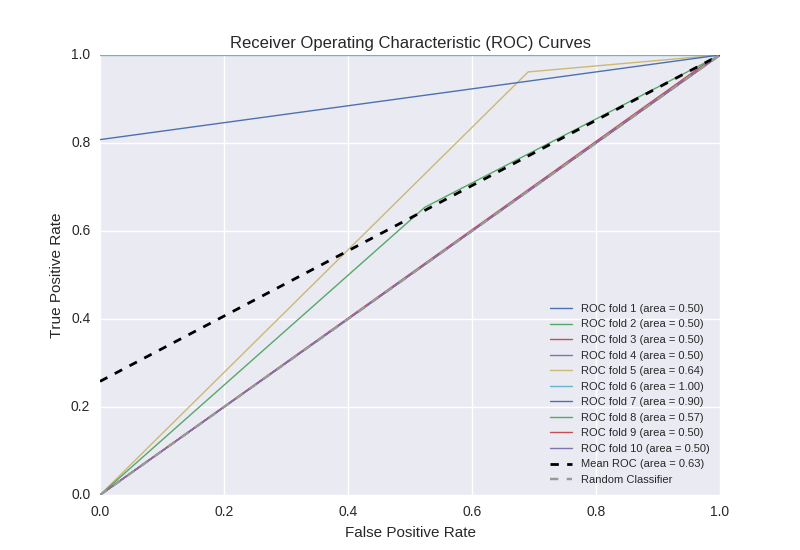
\includegraphics{./Figures/experiments/feat-eng/roc}
     }
	\caption[ROC Curves of a kNN Classifier using Standardization and the Pearson Correlation Filter]{ROC Curves of a kNN Classifier using Standardization and the Pearson Correlation Filter}
	\label{fig:feat-eng-roc-knn-pearson}
\end{figure}

\begin{figure}[H]
	\centering
	\resizebox{\textwidth}{!}{
  	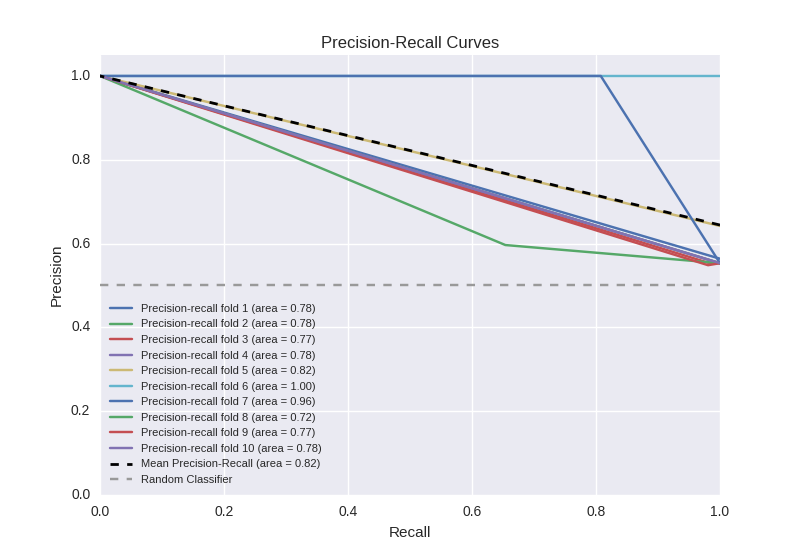
\includegraphics{./Figures/experiments/feat-eng/pr_curve}
     }
	\caption[Precision-Recall Curves of a Naive Bayes Classifier using Standardization and the Pearson Correlation Filter]{Precision-Recall Curves of a Naive Bayes Classifier using Standardization and the Pearson Correlation Filter}
	\label{fig:feat-eng-pr-nb-pearson}
\end{figure}

Although the kNN classifier achieved a score of 0.63, for small rates of false positives ($<0.4$), the number of correctly classified instances is still low. For greater false positive rates, the classifier is able to identify more more instances correctly. Regarding the precision-recall curves, the naive bayes classifier achieved a fairly good result(0.82) for the area under the curve, in some cases with areas greater than 0.90. 

In general, the obtained results provide small improvements over the baseline results. However, the baseline results compete in some cases. Depending on the requirements of the system, one may have to compromise between high precisions or high recalls.

\section{Predicting Relevance through Journalistic Criteria}
\label{sec:jcriteria}

In the previous section we focused on detecting relevance through textual features. Going further, we now describe the process of detecting relevance using an intermediate layer of classifiers. Each intermediate classifier is focused on a single task, i.e., it detects one of the following criteria: controversialness (controversial/not controversial), interestingness (interesting/not interesting), meaningfulness (meaningful/meaningless), novelty (new/old), reliability (reliable/unreliable) and scope (wide/narrow). Each one of these classifiers has as input the textual data and outputs a single prediction of a journalistic aspect. After this, the last classifier receives these journalistic predictions and outputs the final relevance prediction. The intermediate journalistic classifiers start by extracting the same textual features described in table \ref{table-features} with possible preprocessing and feature selection/reduction applied afterwards. The last classifier used these journalistic predictions as its features. Figure \ref{fig:diag-journalistic-criteria} illustrates this idea.
\begin{figure}[H]
	\centering
	\resizebox{\textwidth}{!}{
  	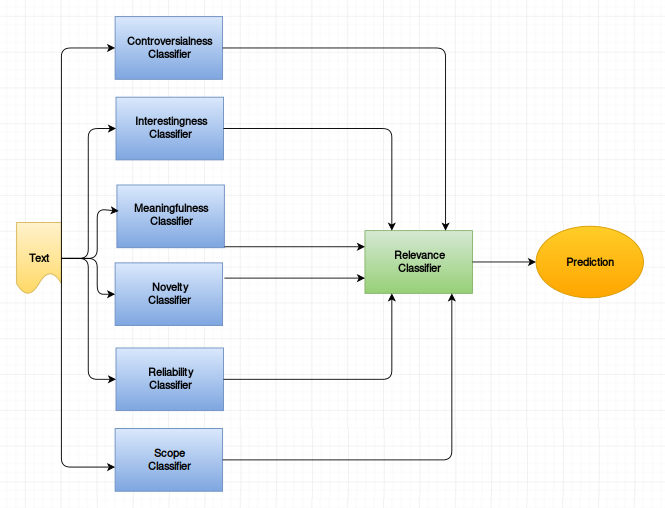
\includegraphics{./Figures/experiments/journalistic-relevance/jr}
     }
	\caption[Prediction of Relevance using Journalistic Criteria]{Prediction of Relevance using Journalistic Criteria}
	\label{fig:diag-journalistic-criteria}
\end{figure}

Table \ref{tab:theoretical-journalistic-relevance-classifiers} shows the results of training the relevance classifier, based on the 6 different, manually annotated journalistic data. The only preprocessing method applied was Standardization. For such a small feature set, we did not apply any feature selection or reduction method, since they did not provide significant improvements. We used a variation of the SVM classifier, which uses a polynomial kernel, with the intent of achieving a better decision boundary that could separate better the classes. Nevertheless, the model parameters were the same as in the baseline experiments. Table \ref{tab:theoretical-journalistic-relevance-classifiers} shows the obtained results.	
\begin{table}[H]
\centering
\small
\resizebox{\textwidth}{!}{%
\begin{tabular}{|l|c|c|c|c|c|c|}
\hline
\multicolumn{1}{|r|}{\textbf{}} & \multicolumn{6}{c|}{\textbf{Training of a Relevance Classifier based on Journalistic Criteria}} \\ \hline
\multicolumn{1}{|r|}{\textbf{Performance Metrics}} & \multirow{2}{*}{\textbf{Accuracy}} & \multirow{2}{*}{\textbf{Precision}} & \multirow{2}{*}{\textbf{Recall}} & \multirow{2}{*}{\textbf{F$_1$}} & \multirow{2}{*}{\textbf{AP}} & \multirow{2}{*}{\textbf{AUC}} \\ \cline{1-1}
\textbf{Classifier} &  &  &  &  &  &  \\ \hline
Minimum Distance Classifier & 0.80 $\pm$ 0.06 & \textbf{0.84 $\pm$ 0.07} & 0.80 $\pm$ 0.08 & 0.82 $\pm$ 0.06 & 0.87 $\pm$ 0.04 & 0.80 $\pm$ 0.06 \\ \hline
K-Nearest Neighbors& \textbf{0.82 $\pm$ 0.07} & 0.82 $\pm$ 0.07 & \textbf{0.86 $\pm$ 0.08}  & \textbf{0.84 $\pm$ 0.06} & \textbf{0.88 $\pm$ 0.04} & \textbf{0.81 $\pm$ 0.07} \\ \hline
Naive Bayes& 0.81 $\pm$ 0.06 & 0.84 $\pm$ 0.07 & 0.81 $\pm$ 0.08 & 0.82 $\pm$ 0.06 & \textbf{0.88 $\pm$ 0.04} & \textbf{0.81 $\pm$ 0.06} \\ \hline
SVM(Linear) & 0.80 $\pm$ 0.06 & 0.82 $\pm$ 0.07 & 0.84 $\pm$ 0.08 & 0.83 $\pm$ 0.06 & 0.87 $\pm$ 0.04 & 0.80 $\pm$ 0.07 \\ \hline
SVM(Polynomial Kernel) & 0.81 $\pm$ 0.06 & 0.82 $\pm$ 0.07 & \textbf{0.86 $\pm$ 0.07} & \textbf{0.84 $\pm$ 0.06} & \textbf{0.88 $\pm$ 0.04} & \textbf{0.81 $\pm$ 0.07} \\ \hline
Decision Tree& 0.79 $\pm$ 0.07 & 0.81 $\pm$ 0.07 & 0.82 $\pm$ 0.08 & 0.81 $\pm$ 0.06 & 0.87 $\pm$ 0.04 & 0.79 $\pm$ 0.07 \\ \hline
Random Forest & 0.80 $\pm$ 0.07 & 0.81 $\pm$ 0.07 & 0.84 $\pm$ 0.07 & 0.82 $\pm$ 0.06 & 0.87 $\pm$ 0.04 & 0.79 $\pm$ 0.07 \\ \hline
\end{tabular}%
}
\caption[Results on predicting Relevance based on Journalistic Criteria]{Results on predicting Relevance based on Journalistic Criteria}
\label{tab:theoretical-journalistic-relevance-classifiers}
\end{table}

From the observed results, it is clear that the SVM with the polynomial kernel and the kNN classifiers achieved the best performance, with the latter achieving a better accuracy(0.82). However, the Minimum Distance Classifier obtained the best overall precision  (0.84). For the rest of the metrics, the SVM with the polynomial kernel and the kNN achieved the overall best recall(0.86), F$_1$ score (0.84), average precision (0.88) and AUC (0.81). The naive bayes also got the best areas under the precision-recall and ROC curves. Figures \ref{fig:theoretical-journalistic-relevance-roc},\ref{fig:theoretical-journalistic-relevance-pr} shows the ROC and Precision-Recall curves. 

\begin{figure}[H]
	\centering
	\resizebox{\textwidth}{!}{
  	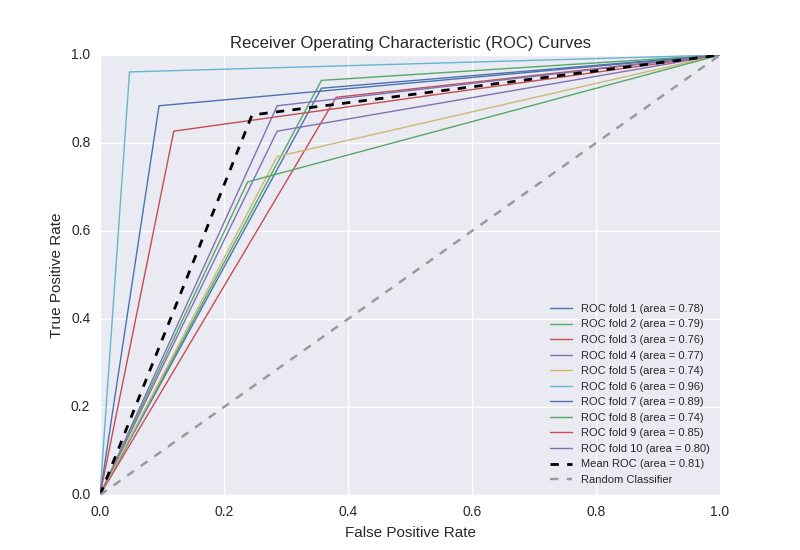
\includegraphics{./Figures/experiments/journalistic-relevance/theoretical/roc}
     }
	\caption[ROC Curves of a Journalistic Based kNN Classifier]{ROC Curves of a Journalistic Based kNN Classifier}
	\label{fig:theoretical-journalistic-relevance-roc}
\end{figure}

\begin{figure}[H]
	\centering
	\resizebox{\textwidth}{!}{
  	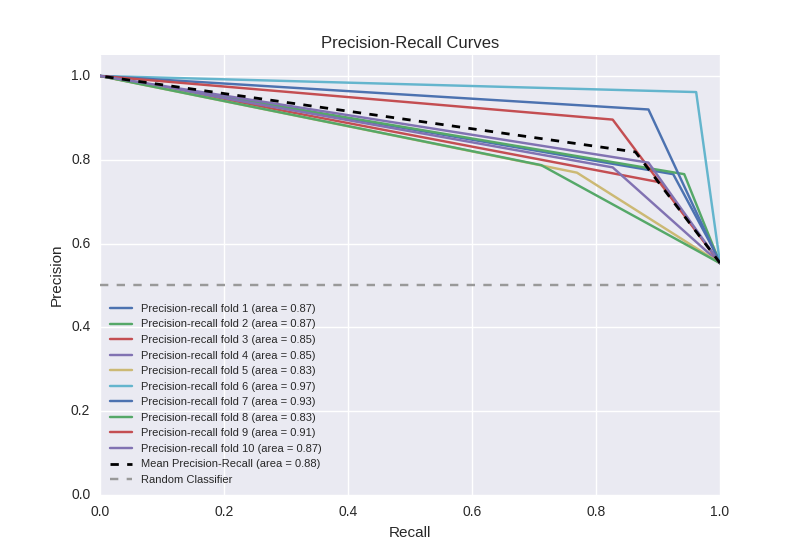
\includegraphics{./Figures/experiments/journalistic-relevance/theoretical/pr_curve}
     }
	\caption[Precision-Recall Curves of a Journalistic Based kNN Classifier]{Precision-Recall Curves of a Journalistic Based kNN Classifier}
	\label{fig:theoretical-journalistic-relevance-pr}
\end{figure}

The kNN classifier achieved a decent area under the ROC curve(0.81), showing that even for low false positive rates such as 0.2, it obtains decent true positive rates($>$ 0.7), on average. Nevertheless, in some cases, it outperformed the AUC mark of 0.85. Regarding the precision-recall curves, it achieved an area of 0.88, on a average, providing a good flexibility with the trade-offs. For high values of recall, it also obtained similar high values of precision. 

Given these results, we decided to use the kNN model as our journalistic based, relevance predictor, since it provided the best performance. As for the intermediate models, we performed 6 experiments, each one consisting of using the best found pipeline(best F$_1$ score) during the feature engineering experiments\ref{sec:feature-engineering} for each classifier. Table \ref{tab:journalistic-relevance-classifiers} details the obtained results.

\begin{table}[H]
\centering
\small
\resizebox{\textwidth}{!}{%
\begin{tabular}{|l|c|c|c|c|c|c|}
\hline
\multicolumn{1}{|r|}{\textbf{}} & \multicolumn{6}{c|}{\textbf{Relevance based on Journalistic Criteria}} \\ \hline
\multicolumn{1}{|r|}{\textbf{Performance Metrics}} & \multirow{2}{*}{\textbf{Accuracy}} & \multirow{2}{*}{\textbf{Precision}} & \multirow{2}{*}{\textbf{Recall}} & \multirow{2}{*}{\textbf{F$_1$}} & \multirow{2}{*}{\textbf{AP}} & \multirow{2}{*}{\textbf{AUC}} \\ \cline{1-1}
\textbf{Intermediate Classifiers} &  &  &  &  &  &  \\ \hline
Minimum Distance Classifiers & 0.62 $\pm$ 0.11 & 0.66 $\pm$ 0.17 & 0.89 $\pm$ 0.19 & 0.72 $\pm$ 0.08 & 0.80 $\pm$ 0.06 & 0.59 $\pm$ 0.13 \\ \hline
K-Nearest Neighbors& 0.54 $\pm$ 0.08 & 0.63 $\pm$ 0.14 & 0.57 $\pm$ 0.17 & 0.57 $\pm$ 0.08 & 0.72 $\pm$ 0.05 & 0.54 $\pm$ 0.09 \\ \hline
Naive Bayes& 0.56 $\pm$ 0.01 & 0.56 $\pm$ 0.01 & \textbf{0.97 $\pm$ 0.03} & 0.71 $\pm$ 0.01 & 0.77 $\pm$ 0.01 & 0.52 $\pm$ 0.01 \\ \hline
Linear SVMs& 0.54 $\pm$ 0.03 & 0.56 $\pm$ 0.02 & 0.89 $\pm$ 0.08 & 0.68 $\pm$ 0.03 & 0.75 $\pm$ 0.02 & 0.50 $\pm$ 0.04 \\ \hline
Decision Trees& 0.55 $\pm$ 0.05 & 0.57 $\pm$ 0.03 & 0.78 $\pm$ 0.11 & 0.65 $\pm$ 0.05 & 0.73 $\pm$ 0.03 & 0.52 $\pm$ 0.05 \\ \hline
Random Forests & \textbf{0.79 $\pm$ 0.07} & \textbf{0.80 $\pm$ 0.08} & 0.84 $\pm$ 0.07 & \textbf{0.82 $\pm$ 0.06} & \textbf{0.86 $\pm$ 0.04} & \textbf{0.78 $\pm$ 0.08} \\ \hline
\end{tabular}%
}
\caption[Results on Predicting Relevance by an Ensemble of Journalistic Classifiers]{Results on Predicting Relevance by an Ensemble of Journalistic  Classifiers}
\label{tab:journalistic-relevance-classifiers}
\end{table}

Random forests revealed to be the best option for the intermediate classifiers. They achieved the best accuracy(0.79), precision(0.80) and F$_1$(0.82) score. However, the naive bayes obtained an outstanding value for recall of 0.97. Regarding the areas below the ROC and precision-recall curves, the Random Forests also achieved the best values, obtaining 0.78 and 0.86, respectively. Figures \ref{fig:rt-journalistic-relevance-roc} and \ref{fig:rt-journalistic-relevance-pr} show the ROC and precision-recall curves, respectively.

\begin{figure}[H]
	\centering
	\resizebox{\textwidth}{!}{
  	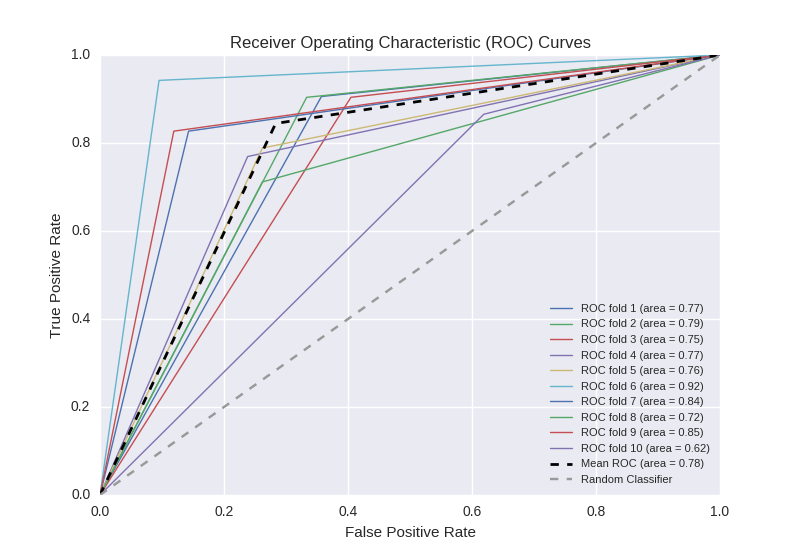
\includegraphics{./Figures/experiments/journalistic-relevance/rt/roc2}
     }
	\caption[ROC Curves of a Journalistic Based kNN Classifier, using Random Forests for the intermediate classifiers]{ROC Curves of a Journalistic Based kNN Classifier, using Random Forests for the intermediate classifiers}
	\label{fig:rt-journalistic-relevance-roc}
\end{figure}

\begin{figure}[H]
	\centering
	\resizebox{\textwidth}{!}{
  	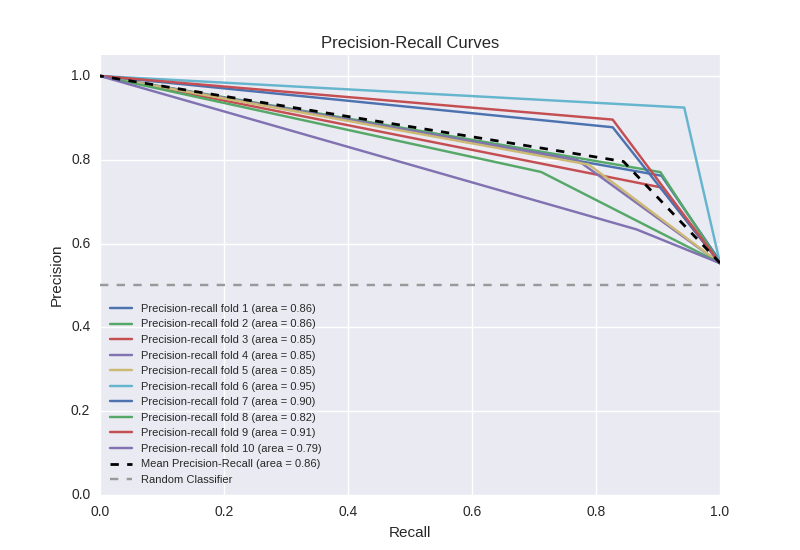
\includegraphics{./Figures/experiments/journalistic-relevance/rt/pr_curve2}
     }
	\caption[Precision-Recall Curves of a Journalistic Based kNN Classifier, using Random Forests for the intermediate classifiers]{Precision-Recall Curves of a Journalistic Based kNN Classifier, using Random Forests for the intermediate classifiers}
	\label{fig:rt-journalistic-relevance-pr}
\end{figure}

The classifier got a good mean area under the ROC curve(0.78), meaning that is able to identify and classify correctly most of the instances, even for low false positive rates. Regarding the precision-recall graph, which has a good area under the mean curve(0.85), the classifier consistently shows high values of precision, even when the recall increases.

Comparing with the initial baseline experiments, the general scenario is fairly better. There was an improvement in accuracy of 15\%, 8\% in precision and recall, 9\% in F$_1$, 6\% in average precision and 16\% in AUC.

\section{Discussion}

The obtained results suggest that using a meta classifier that makes use of an intermediate tier of the best single strong models is the preferred method. By using a Random Forest classifier to predict each one of the journalistic criteria, and a kNN classifier to detect the final relevance, it was possible to achieve the best accuracy(0.79), precision(0.80) and F$_1$ (0.82) score. In fact, seeing different aspects of the problem space (different criteria) was helpful to reduce the generalization error and variance. This method proved to be a good choice to be used in the REMINDS system. \\
Although with different goals, other system achieved similar F$_1$ performances, such as predicting spam or not spam(0.79) \citep{Irani2010TrendStuff} by using a Decision Tree (C4.5). Simiraly, Liparas et al.\citep{Liparas2014NewsClassification} achieved a F$_1$ score of 0.85 by using simple bigrams and metadata from the tweets, with a Naive Bayes, to classify web pages by topic. Fernandes et al. \citep{Fernandes2015PredictingPopularity} also used a Random Forest to predict the popularity of a web article, obtaining a F$_1$ score of 0.69.




